\documentclass[spanish,a4paper,12pt,oneside]{extreport}

\usepackage[dvips]{graphicx}
\usepackage[dvips]{epsfig}
\usepackage[utf8]{inputenc}
\usepackage[spanish]{babel}
\usepackage{alltt}

\usepackage[ruled,vlined,commentsnumbered,linesnumbered,inoutnumbered,titlenotnumbered,noend]{algorithm2e}
\SetKwRepeat{Do}{do}{while}

\usepackage{multirow}
\usepackage{array} 
\usepackage{amsfonts}
\usepackage{amsmath}
\usepackage{bigstrut}
\usepackage{booktabs}
\usepackage{caption}
\usepackage{chngpage}
\usepackage{float}
\usepackage{enumitem,lipsum}
\usepackage{graphicx}
\usepackage{lscape}
\usepackage{microtype}
\usepackage[numbers]{natbib}
\usepackage{pdflscape}
\usepackage{rotating}
\usepackage{subcaption}
\usepackage{ctable}
\usepackage{hyperref}
%\usepackage{enumerate} %deprecated
\usepackage{gensymb}
\usepackage{eurosym}
\usepackage{xcolor}
\usepackage{tabu}

\usepackage{lineno}
%\\linenumbers
%\setlength\linenumbersep{5pt}
%\renewcommand\linenumberfont{\normalfont\tiny\sffamily\color{gray}}

% TABLES

% END TABLES

\usepackage[top=2cm, bottom=2cm, left=2cm, right=2cm]{geometry}

\newenvironment{sourcecode}
{\begin{list}{}{\setlength{\leftmargin}{1em}}\item\scriptsize\bfseries}
{\end{list}}

\newenvironment{littlesourcecode}
{\begin{list}{}{\setlength{\leftmargin}{1em}}\item\tiny\bfseries}
{\end{list}}

\newenvironment{summary}
{\par\noindent\begin{center}\textbf{Abstract}\end{center}\begin{itshape}\par\noindent}
{\end{itshape}}

\newenvironment{keywords}
{\begin{list}{}{\setlength{\leftmargin}{1em}}\item[\hskip\labelsep \bfseries Keywords:]}
{\end{list}}

\newenvironment{palabrasClave}
{\begin{list}{}{\setlength{\leftmargin}{1em}}\item[\hskip\labelsep \bfseries Palabras clave:]}
{\end{list}}

\usepackage{bera}% optional: just to have a nice mono-spaced font
\usepackage{listings}
\usepackage{xcolor}

\colorlet{punct}{red!60!black}
\definecolor{background}{HTML}{EEEEEE}
\definecolor{delim}{RGB}{20,105,176}
\colorlet{numb}{magenta!60!black}

\lstdefinelanguage{json}{
    basicstyle=\normalfont\ttfamily,
    numbers=left,
    numberstyle=\scriptsize,
    stepnumber=1,
    numbersep=8pt,
    showstringspaces=false,
    breaklines=true,
    frame=lines,
    backgroundcolor=\color{background},
    literate=
     *{0}{{{\color{numb}0}}}{1}
      {1}{{{\color{numb}1}}}{1}
      {2}{{{\color{numb}2}}}{1}
      {3}{{{\color{numb}3}}}{1}
      {4}{{{\color{numb}4}}}{1}
      {5}{{{\color{numb}5}}}{1}
      {6}{{{\color{numb}6}}}{1}
      {7}{{{\color{numb}7}}}{1}
      {8}{{{\color{numb}8}}}{1}
      {9}{{{\color{numb}9}}}{1}
      {:}{{{\color{punct}{:}}}}{1}
      {,}{{{\color{punct}{,}}}}{1}
      {\{}{{{\color{delim}{\{}}}}{1}
      {\}}{{{\color{delim}{\}}}}}{1}
      {[}{{{\color{delim}{[}}}}{1}
      {]}{{{\color{delim}{]}}}}{1},
}

\begin{document}

\renewcommand\listtablename{Índice de Tablas}    
\renewcommand\listfigurename{Índice de Figuras}    

%%%%%%%%%%%%%%%%%%%%%%%%%%%%%%%%%%%%%%%%%%%%%%%%%%%%%%%%%%%%%%%%%%%%%%%%%%%%%%%
% First Page
%%%%%%%%%%%%%%%%%%%%%%%%%%%%%%%%%%%%%%%%%%%%%%%%%%%%%%%%%%%%%%%%%%%%%%%%%%%%%%%
\pagestyle{empty}
\thispagestyle{empty}


\newcommand{\HRule}{\rule{\linewidth}{1mm}}
\setlength{\parindent}{0mm}
\setlength{\parskip}{0mm}

\vspace*{\stretch{0.5}}

\begin{center}

\includegraphics[scale=0.8]{images/escuela-ingenieria-tecnologia-original}\\[10mm]
{\Huge Trabajo de Fin de Grado}
\end{center}

\HRule
\begin{flushright}
        {\Huge Predicción de series temporales meteorológicas mediante técnicas de aprendizaje profundo } \\[2.5mm]
        {\Large \textit{Weather time series forecasting using deep learning techniques}} \\[5mm]
        {\Large José Ramón Morera Campos} \\[5mm]


\end{flushright}
\HRule
\vspace*{\stretch{2}}
\begin{center}
  \Large La Laguna, \today
\end{center}

\setlength{\parindent}{5mm}

%%%%%%%%%%%%%%%%%%%%%%%%%%%%%%%%%%%%%%%%%%%%%%%%%%%%%%%%%%
% Signature page (add the official stamp)
%%%%%%%%%%%%%%%%%%%%%%%%%%%%%%%%%%%%%%%%%%%%%%%%%%%%%%%%%%
\newpage
\thispagestyle{empty}

D. {\bf Leopoldo Acosta Sánchez}, profesor Catedrático de Universidad adscrito al Departamento de Ingeniería Informática y de Sistemas de la Universidad de La Laguna, como tutor

\bigskip
D. {\bf Daniel Acosta Hernández}, Ingeniero Informático adscrito al Departamento de Ingeniería Informática y de Sistemas de la Universidad de La Laguna en calidad de estudiante de doctorado, como tutor

\pagestyle{empty}

\bigskip
\bigskip
{\bf C E R T I F I C A N}

\bigskip
\bigskip
Que la presente memoria titulada:

\bigskip
''{\it Predicción de series temporales mediante técnicas de aprendizaje profundo}''

\bigskip
\bigskip
\bigskip

\noindent ha sido realizada bajo su dirección por D. {\bf José Ramón Morera Campos}.

\bigskip
\bigskip

Y para que así conste, en cumplimiento de la legislación vigente y a los efectos
oportunos firman la presente en La Laguna a \today

%%%%%%%%%%%%%%%%%%%%%%%%%%%%%%%%%%%%%%%%%%%%%%%%%%%%%%%%%%
\newpage
\thispagestyle{empty}

{ \begin{LARGE}
Agradecimientos
\end{LARGE}

\hspace{3mm}

\begin{large}
Quisiera agradecer a todas las personas que han contribuido de forma directa o indirecta a la realización de este Trabajo de Fin de Grado. \\

En primer lugar, agradezco a mis tutores, Leopoldo Acosta y Daniel Acosta, por su orientación y disponibilidad a lo largo del desarrollo del trabajo. 
Su apoyo ha sido fundamental para alcanzar los objetivos propuestos. \\

También deseo expresar mi agradecimiento a los profesores y al personal de la Universidad por la formación recibida durante estos años, que se ve reflejada en este proyecto final. \\

Agradezco igualmente a mis compañeros y compañeras de grado por su colaboración y por el intercambio de ideas y experiencias que enriquecieron el proceso de aprendizaje. \\

Por último, quiero reconocer el apoyo de mi familia durante este periodo, así como de todas aquellas personas que, de una u otra forma, han hecho posible la finalización de esta etapa académica. \\
\end{large}

}
%%%%%%%%%%%%%%%%%%%%%%%%%%%%%%%%%%%%%%%%%%%%%%%%%%%%%%%%
\newpage
\thispagestyle{empty}

\bigskip
\begin{LARGE}
Licencia
\end{LARGE}

\bigskip
\bigskip
\bigskip
\bigskip

\begin{center}

\includegraphics[scale=1.8]{images/by-nc-nd_88x31}\\[5mm]
\end{center}

\begin{large}
© Esta obra está bajo una licencia de Creative Commons Reconocimiento-NoComercial-SinObrasDerivadas 4.0 Internacional.
\end{large}

%%%%%%%%%%%%%%%%%%%%%%%%%%%%%%%%%%%%%%%%%%%%%%%%%%%%%%%%
\newpage 
\thispagestyle{empty}

\begin{abstract}
{\em
Este trabajo presenta el desarrollo de un sistema de predicción a corto plazo de series temporales meteorológicas, basado en técnicas de aprendizaje profundo, 
utilizando datos procedentes de múltiples estaciones meteorológicas de la isla de Tenerife. El objetivo principal es diseñar y
evaluar modelos capaces de generalizar a ubicaciones nuevas, no vistas durante el entrenamiento, sin necesidad de reentrenamiento. Este enfoque corresponde al
problema conocido como zero-shot, un ámbito aún poco explorado en la literatura de predicción de series temporales.

Se estudian distintas arquitecturas de redes neuronales, incluyendo modelos LSTM, CNN y un híbrido CNN-LSTM, comparándolos con enfoques tradicionales como ARIMA.
Se lleva a cabo un exhaustivo proceso de preprocesamiento de datos, que incluye la imputación de valores faltantes, codificación temporal y normalización,
así como la construcción de conjuntos de datos mediante ventanas deslizantes. Además, se realizan diversos experimentos para explorar técnicas y configuraciones
tanto en el tratamiento de los datos como en la arquitectura de los modelos, con el objetivo de optimizar los resultados.

Los experimentos muestran que los modelos LSTM alcanzan una alta precisión en horizontes de predicción cortos, superando a los modelos convencionales.
Finalmente, se implementa una aplicación web que permite a los usuarios generar pronósticos a partir de datos en tiempo real.
El sistema demuestra ser modular, escalable y con potencial para su aplicación práctica.

}

\begin{palabrasClave}
predicción de series temporales, aprendizaje profundo, redes neuronales, LSTM, meteorología
\end{palabrasClave}

\end{abstract}
%%%%%%%%%%%%%%%%%%%%%%%%%%%%%%%%%%%%%%%%%%%%%%%%%%%%%%%%%
\newpage 
\vspace*{200px}
\thispagestyle{empty}

\begin{summary}
{
This work presents the development of a short-term prediction system for meteorological time series, based on deep learning techniques, using data from multiple weather stations on the island of Tenerife. The main objective is to design and evaluate models capable of generalizing to new locations, not seen during training, without the need for retraining. This approach corresponds to the problem known as zero-shot, a domain still scarcely explored in the time series prediction literature.

Different neural network architectures are studied, including LSTM, CNN, and a CNN-LSTM hybrid model, comparing them with traditional approaches such as ARIMA. A thorough data preprocessing process is carried out, which includes missing value imputation, temporal encoding, and normalization, as well as the construction of datasets using sliding windows. Additionally, various experiments are conducted to explore techniques and configurations both in data treatment and model architecture, aiming to optimize the results.

The experiments show that LSTM models achieve high accuracy in short-term prediction horizons, outperforming conventional models. Finally, a web application is implemented that allows users to generate forecasts based on real-time data. The system proves to be modular, scalable, and with potential for practical application.
}

\em
\begin {keywords}
time series forecasting, deep learning, neural networks, LSTM, weather prediction
\end {keywords}

\end{summary}
%%%%%%%%%%%%%%%%%%%%%%%%%%%%%%%%%%%%%%%%%%%%%%%%%%%%%%%%%
\newpage{\pagestyle{empty}}
\thispagestyle{empty}

%%%%%%%%%%%%%%%%%%%%%%%%%%%%%%%%%%%%%%%%%%%%%%%%%%%%%%%%%
\pagestyle{myheadings} %my head defined by markboth or markright
% No funciona bien \markboth sin \char`\"twoside\char`\" en \documentclass, pero al
% ponerlo se dan un montón de errores de underfull \vbox, con lo que no se
% ha puesto.


%%Aqui debería poner el nombre del proyecto pero, como es muy grande no cabe y se ve feo en el PDF
\markboth{xxxxx}{}

%%%%%%%%%%%%%%%%%%%%%%%%%%%%%%%%%%%%%%%%%%%%%%%%%%%%%%%%%
%Numeracion en romanos
\renewcommand{\thepage}{\roman{page}}
\setcounter{page}{1}
\pagestyle{plain} 

%%%%%%%%%%%%%%%%%%%%%%%%%%%%%%%%%%%%%%%%%%%%%%%%%%%%%%%%%

\tableofcontents

%%%%%%%%%%%%%%%%%%%%%%%%%%%%%%%%%%%%%%%%%%%%%%%%%%%%%%%%%
\newpage{\pagestyle{empty}}

\listoffigures

%%%%%%%%%%%%%%%%%%%%%%%%%%%%%%%%%%%%%%%%%%%%%%%%%%%%%%%%%
\newpage{\pagestyle{empty}}

\listoftables

%%%%%%%%%%%%%%%%%%%%%%%%%%%%%%%%%%%%%%%%%%%%%%%%%%%%%%%%%%%%%%%%%%%%%%%%%%%%%%%
\newpage{\pagestyle{empty}}

%%%%%%%%%%%%%%%%%%%%%%%%%%%%%%%%%%%%%%%%%%%%%%%%%%%%%%%%%%%%%%%%%%%%%%%%%%%%%%%
\newpage
\thispagestyle{empty}

%Numeracion a partir del capitulo I
\renewcommand{\thepage}{\arabic{page}}
\setcounter{page}{1}
\pagestyle{plain}

\chapter{\LARGE Introducción}
\label{chapter:intro}

\section{Motivación del proyecto}
La predicción de series temporales es un campo de estudio que ha cobrado gran relevancia en los últimos años, especialmente en el ámbito del aprendizaje automático y el aprendizaje profundo. 
La capacidad de anticipar eventos futuros a partir de datos históricos es fundamental en diversas áreas, como la economía, la meteorología, la salud y la ingeniería. 

El campo de la meteorología, en particular, ha aumentado su relevancia en los útlimos años debido al aumento de fenómenos climáticos extremos y su impacto en la sociedad. 
Prever con antelación la evolución de variables meteorológicas no solo permite planificar recursos, sino también contribuir a la prevención de desastres naturales.

En este contexto, el uso de redes neuronales ha demostrado ser una herramienta poderosa para abordar problemas complejos de predicción.
Gracias a los avances en capacidad de cómputo y la disponibilidad de grandes volúmenes de datos, arquitecturas como LSTM, GRU y Transformers se han consolidado como soluciones de alto rendimiento. 
Estas redes no solo capturan patrones temporales de manera eficiente, sino que también pueden adaptarse dinámicamente a cambios en el comportamiento de la serie, mejorando la precisión y la robustez de las predicciones.


\section{Planteamineto}
En este trabajo se pretende emplear mediciones de múltiples estaciones meteorológicas de la isla de Tenerife con el fin de desarrollar un modelo de predicción climatológica a corto plazo.
Se busca que dicho modelo sea capaz de generalizar más allá de las estaciones de entrenamiento. Esto es, que a partir de mediciones meteorológicas de cualquier origen, el modelo sea capaz de 
generar predicciones a corto plazo (3, 6 o 12 horas) de gran calidad.
Se deciden considerar 3 variables meteorológicas: temperatura, humedad y presión atmosférica.
La elección de estas variables se basa en su relevancia para la predicción del clima y la existencia de registros en las estaciones meteorológicas de Tenerife.

Se establece un especial énfasis en el tratamiento de los datos, estudiándose exhaustivamente diversas técnicas.

La idea principal pasa por la creación de ventanas de información, que son secuencias de datos consecutivos agrupados 

Como parte del trabajo se contempla el despliegue de una infraestructura tecnológica que permita la captura y el procesamiento de datos públicos,
 así como la creación y evaluación de diversos modelos predictivos que extraigan información valiosa a partir de estos datos.
 
Para ello, se emplará el lenguaje de programación Python, que ofrece una amplia gama de bibliotecas y herramientas para el análisis de datos y la 
implementación de modelos de aprendizaje automático.

Así mismo, se plantea desplegar los modelos en un entorno de producción, permitiendo su uso en aplicaciones prácticas. 
De esta forma, cualquier usuario podrá suministrar mediciones de la variable que desee durante las últimas horas y obtener un pronóstico.

\section{Antecedentes y estado del arte}

El uso de redes neuronales y técnicas de deep learning (aprendizaje profundo) para la predicción de series temporales tiene sus orígenes en la década de 1940. Aunque el término deep learning ha ganado relevancia en los últimos años, los conceptos fundamentales y algunas de las técnicas más empleadas han existido desde hace mucho tiempo, evolucionando y perfeccionándose con el avance de la tecnología.
En 1943, Warren McCulloch y Walter Pitts fueron pioneros en desarrollar un modelo computacional para redes neuronales \cite{mcculloch1943}, 
estableciendo las bases de lo que hoy conocemos como inteligencia artificial basada en redes neuronales. 
Más adelante, en 1949, Donald Hebb introdujo la famosa Teoría Hebbiana, una hipótesis que proponía un mecanismo de aprendizaje basado en la plasticidad neuronal \cite{hebb1949}. 
Este principio se aplicó a modelos computacionales, impulsando la investigación en la simulación del aprendizaje humano.


En 1958, Frank Rosenblatt avanzó en este campo con la creación del perceptrón \cite{rosenblatt1958}, un algoritmo pionero de reconocimiento de patrones basado en una red de aprendizaje de computadora de dos capas.
Este modelo simple operaba mediante operaciones de adición y sustracción, sentando las bases para el desarrollo de redes neuronales más complejas.
Durante las siguientes décadas, la investigación en redes neuronales experimentó un estancamiento debido a limitaciones técnicas y a la falta de métodos eficaces para el entrenamiento de redes con múltiples capas. 
Sin embargo, en 1982, un gran avance revitalizó este campo: la introducción del algoritmo de propagación hacia atrás (backpropagation) \cite{werbos1982}, que resolvía el problema del entrenamiento eficiente de redes neuronales profundas, 
permitiendo la formación de redes multicapa de manera más rápida y eficaz.
Desde entonces, las redes neuronales han continuado evolucionando, impulsadas en gran parte por los avances en la potencia de cálculo de las GPU y el desarrollo del deep learning.
Hoy en día, esta tecnología es fundamental y revolucionaria, capaz de realizar predicciones de series temporales con notable rapidez y precisión.
La investigación en este ámbito sigue siendo prolífica. Una búsqueda rápida en internet revela la continua producción de proyectos y estudios enfocados 
en perfeccionar las técnicas de predicción temporal mediante aprendizaje profundo. Estos trabajos se caracterizan por un análisis exhaustivo y la exploración de nuevos métodos, 
todos con el objetivo de optimizar la precisión y la eficacia de las previsiones en aplicaciones prácticas.

\section{Objetivos}

\begin{enumerate}[label=\arabic*.] 
    \item Evaluar y seleccionar una fuente de datos.
    \item Evaluar y seleccionar el framework de aprendizaje profundo a usar en el proyecto.
    \item Diseño e implementación de la metodología de procesamiento de los datos.
    \item Evaluación y selección de arquitecturas pertinentes al problema.
    \item Implementación de una arquitectura adecuada.
    \item Evaluación del rendimiento de la solución propuesta.
    \item Comparación frente a metodologías tradicionales.
    \item Despliegue de la solución en un entorno de producción.
\end{enumerate}

\newpage


%%%%%%%%%%%%%%%%%%%%%%%%%%%%%%%%%%%%%%%%%%%%%%%%%%%%%%%%%%%%%%%%%%%%%%%%%%%%%%%
\newpage{\pagestyle{empty}}
\thispagestyle{empty}

\chapter{\LARGE Adquisición y preprocesado de datos}
\label{chapter:dos}


Se desea trabajar con series temporales sobre mediciones climatológicas. 
En concreto, se eligen las variables de temperatura del aire, humedad relativa y presión atmosférica en la superficie.
Dichas variables son estudiadas con frecuencia horaria, en el intervalo comprendido entre el 1 de marzo de 2023 y el 28 de febrero de 2025.

Es imprescindible disponer de un conjunto de datos que abarque un período de tiempo suficientemente amplio para poder cubrir las diversas condiciones climáticas que pueden presentarse.
Además, es relevante el uso de datos en un período múltiplo del año, para asegurar que se capturan las variaciones estacionales y que el conjunto de datos está suficientemente equilibrado.
Es decir, si se emplearan un año y 3 meses, se podría sesgar el conjunto introduciendo más días con temperaturas bajas, por ejemplo, si se cubrieran 2 inviernos pero un solo verano.

\section{Fuentes de los datos}

Se han empleado 2 fuentes para recopilar las mediciones: 
\begin{itemize}
    \item \textbf{Grafcan}: Cartográfica de Canarias, S.A. es una empresa pública de la Comunidad Autónoma de Canarias. Dispone de una red de estaciones meteorológicas cuyas
    mediciones son accesibles mediante una API REST de acceso gratuito previa solicitud de una clave\cite{grafcan_sensores}. 
    \item \textbf{Open-Meteo}: API pública de código abierto que proporciona datos de múltiples proveedores de meteorología. Este servicio no dispone de estaciones de medición
    propias, sino que recopila pronósticos de diferentes modelos de predicción climatológica. 

    Se emplea la API de predicciones pasadas\cite{open_meteo_api}. Se seleccionan los modelos ICON Global del servicio meteorológico alemán (DWD) y el modelo ARPEGE Europe de Météo-France. Ambos modelos se actualizan cada 3 horas. 
    Se explora la posibilidad de emplear as predicciones del modelo HAROME de la AEMET, pero no están disponibles de forma pública
\end{itemize}

Se eligen 4 ubicaciones de la isla de Tenerife con distintas características climáticas para el conjunto de entrenamiento y evaluación:
\begin{itemize}
    \item \textbf{San Cristóbal de La Laguna 1 (A)}: La Cuesta, 35 metros de altitud.
    \item \textbf{San Cristóbal de La Laguna 2 (B)}: La Punta del Hidalgo, 54m.
    \item \textbf{La Orotava (C)}: Camino de Chasna, 812m.
    \item \textbf{Arona (D)}: Punta de Rasca, 25m.
\end{itemize}

Así mismo, se escogen 2 ubicaciones para el conjunto de test, nunca vistas en el ajuste del modelo:
\begin{itemize}
    \item \textbf{Garachico (E)}: La Montañeta, 922 m.
    \item \textbf{Santa Cruz de Tenerife (F)}: Polígono Costa Sur, 92m.
\end{itemize}

Las ubicaciones han sido elegidas al contar con estaciones de medición de Grafcan.
Sus posiciones se muestran en la Figura \ref{mapa_estaciones}, con la letra indicada en la lista.
Se señaladan en rojo las estaciones de entrenamiento y en naranja las de test.

\begin{figure}[htb]
   \centering
   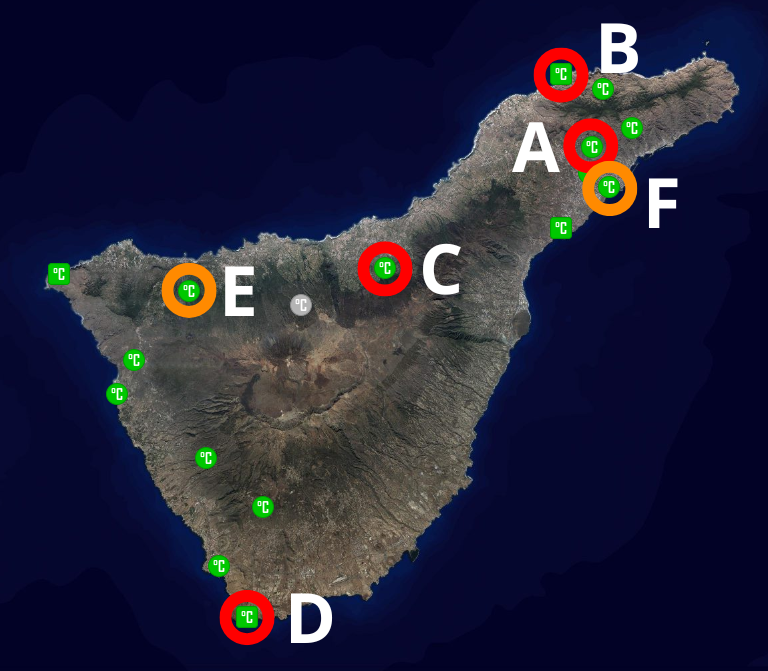
\includegraphics[width=0.6\linewidth]{images/mapa_estaciones}
   \caption{Mapa de las estaciones climatológicas Grafcan empleadas.}
   \label{mapa_estaciones}
\end{figure}

Inicialmente se valoró emplear las estaciones correspondientes a Los Cristianos, Santiago del Teide o la Punta de Teno, pero fueron descartadas por dos motivos: 
se detectó que existían períodos prolongados con datos faltantes en las mediciones de Grafcan. Algunas de ellas también exhibían poca correlación entre las mediciones
del servicio Grafcan y las de Open-Meteo, lo que podría afectar la calidad de los datos.

\bigskip

\section{Proceso de adquisición y almacenamiento}

Para automatizar la adquisición de datos, se emplea la herramienta de orquestación node-red, que permite crear flujos de información mediante nodos que realizan tareas específicas o ejecutan códgio de JavaScript.
En dicha herramienta se desarrollan dos paneles, uno para cada fuente de datos. 
Así mismo, dentro de cada panel se desarrollan dos flujos, uno para la adquisición de datos en un intervalo dado, y otro para la adquisición de datos en tiempo real, en particular, 
se establece la recogida de datos cada 6 horas.

\subsection{Flujos de adquisición de Grafcan}
Debido al funcionamiento de la API de Grafcan, se debe realizar una llamada para obtener la serie temporal de cada variable meteorológica de cada estación.
Posteriormente, se unen las series de cada estación en una única serie, que se almacena en una base de datos PostgreSQL. Este flujo está reflejado en la figura \ref{grafcan_flows}.
\begin{figure}[htb]
   \centering
   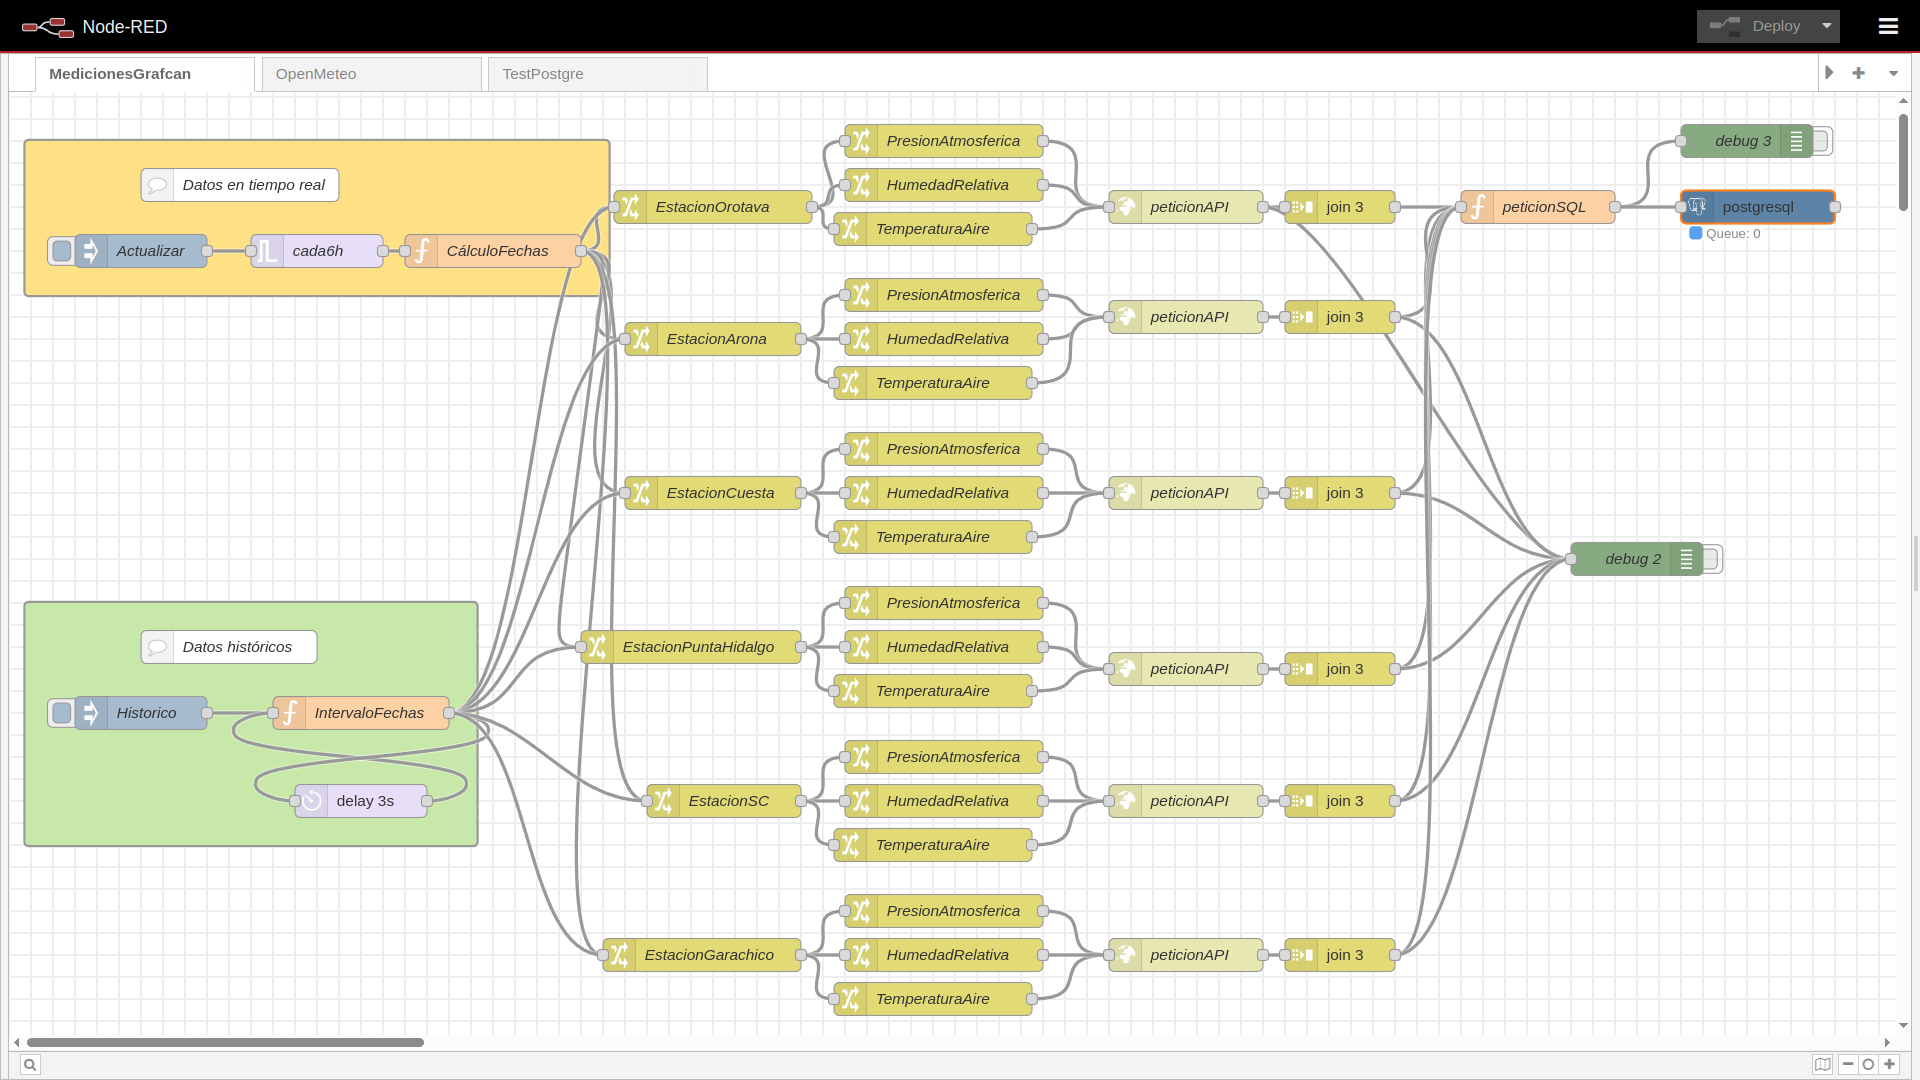
\includegraphics[width=1\linewidth]{images/node-red_grafcan.png}
   \caption{Flujo de adquisición de datos de Grafcan en node-red.}
   \label{grafcan_flows}
\end{figure}

Las mediciones de Grafcan se recogen apróximamente cada 10 minutos, si bien la frecuencia no es consistente y en ocasiones es mayor. Así mismo, 
los instantes de medición son independientes entre las variables estudiadas. Para manejar esta variabilidad, 
en este nivel los datos se agregan cada 10 minutos, usando la media de las mediciones del intervalo.

\subsection{Flujos de adquisición de Open-Meteo}
Existe una rama para obtener los datos del modelo ICON y otra para el modelo ARPEGE. Se establecen las coordenadas de cada ubicación como las de la estación de Grafcan seleccionada 
y se realiza una llamada a la API por cada localización y cada modelo, como se observa en la figura \ref{open-meteo_flows}. 
Los resultados se almacenan en una base de datos PostgreSQL.
\begin{figure}[htb]
   \centering
   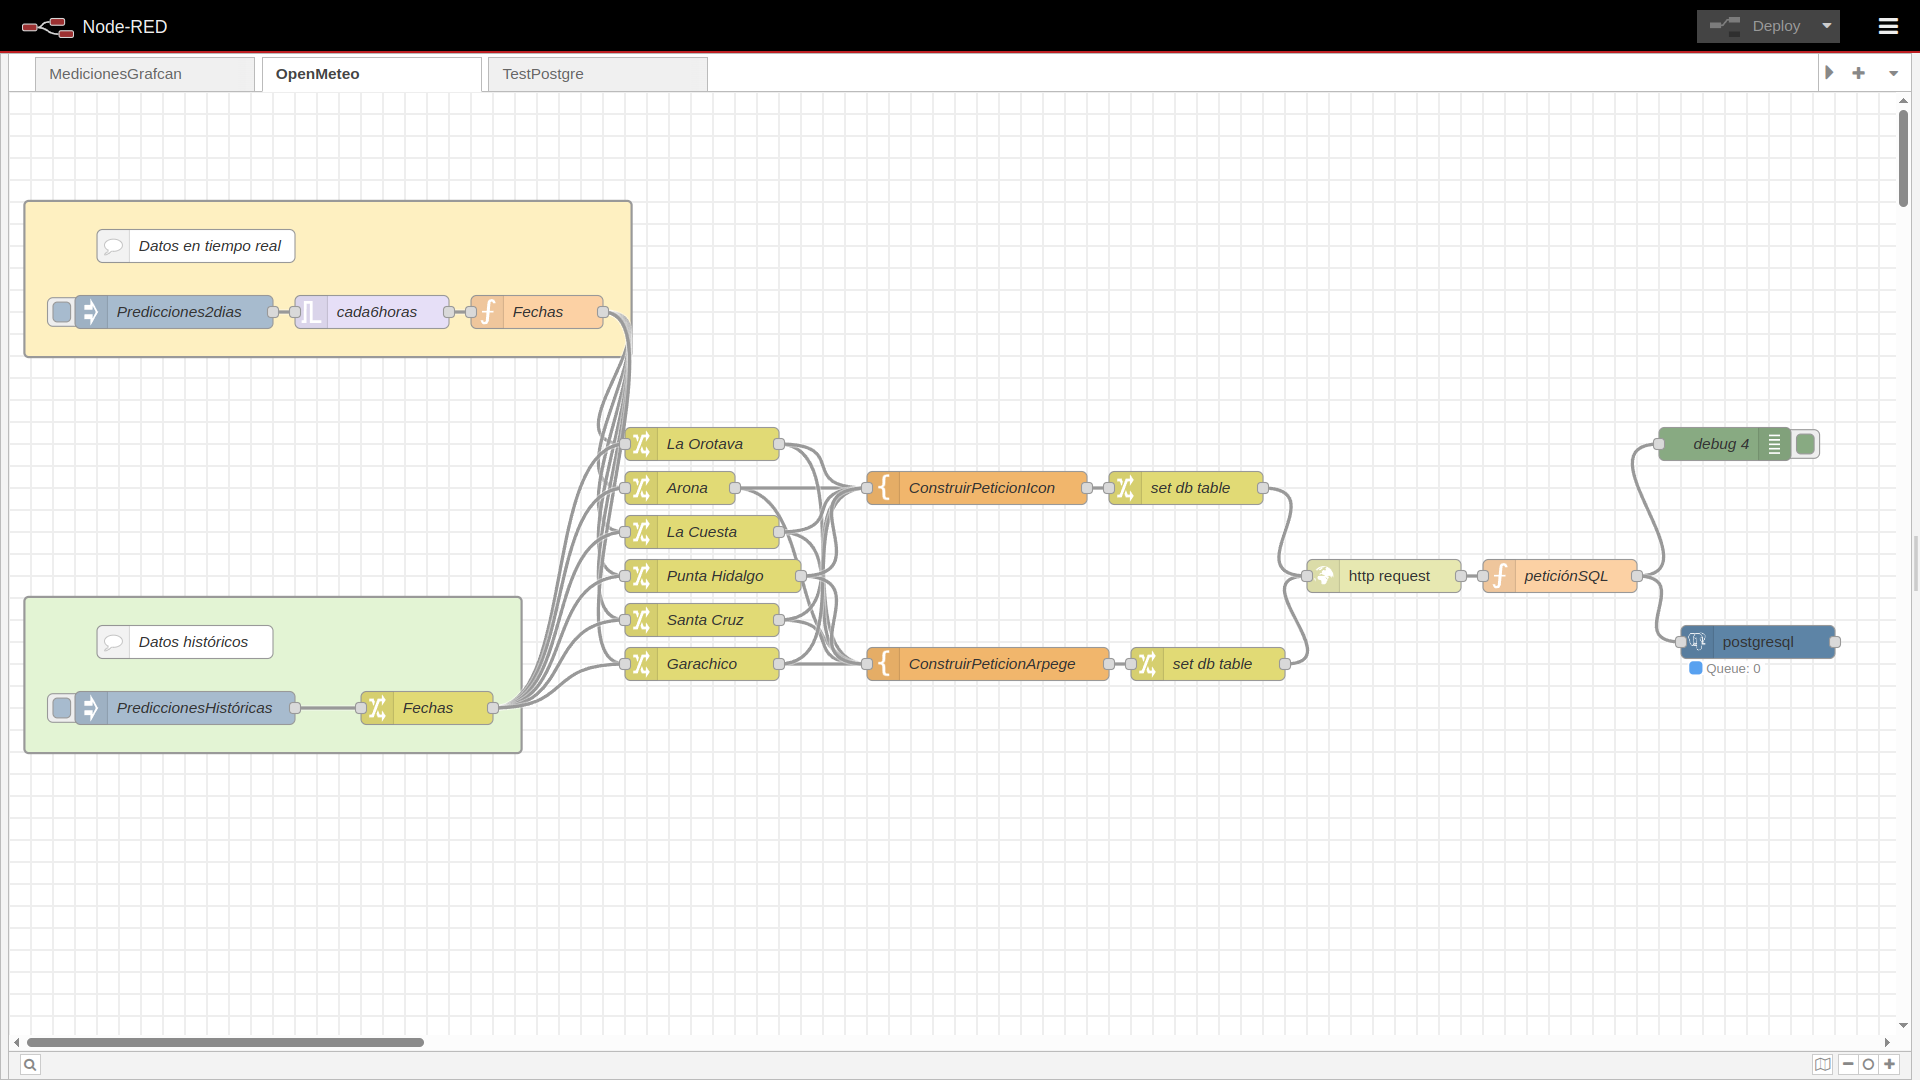
\includegraphics[width=1\linewidth]{images/node-red_open-meteo.png}
   \caption{Flujo de adquisición de datos de Open-Meteo en node-red.}
   \label{open-meteo_flows}
\end{figure}

\subsection{Almacenamiento}
Se estudian distintas alternativas para el almacenamiento de los datos, fundamentalmente, servicios de bases de datos como Redis, MongoDB o PostgreSQL.
Tras valorar las opciones, se opta por emplear TimescaleDB, una extensión del popular sistema PostgreSQL
de bases de datos relacionales, especialmente adaptada para el manejo de series temporales. 

Se establece un servidor TimescaleDB en un contenedor Docker. Se configura una tabla para cada estación y cada fuente: Grafcan, Open-Meteo ICON y Open-Meteo ARPEGE. 
Cada tabla emplea como índice y clave primaria la fecha y hora de la medición, así como su zona horaria. Las otras columnas se corresponden a la temperatura media del aire
 en grados Celsius, la humedad relativa en porcentaje y la presión atmosférica en superficie medida en hPa.

Es importante señalar que las mediciones de Grafcan y Open-Meteo codifican las horas en UTC, en vez de la hora local, puesto que UTC es independiente a los cambios de horario
y de esta forma se mantiene la consistencia de los datos.

\section{Preprocesado}

Se desarrolla un cuaderno de Jupyter para realizar el preprocesado de los datos. El proceso descrito en este apartado
se aplica de forma separada para cada ubicación.

En primer lugar, se obtienen las series temporales de las 3 fuentes: Grafcan y los dos modelos de Open-Meteo, para el período entre el 1 de marzo de 2023 y el 28 de febrero de 2025.
Se agregan los datos con frecuencia horaria mediante la media. 

\textbf{Nota:} En la estación de Garachico, usada para el test, el período empleado es del 1 de marzo de 2024 al 28 de febrero de 2025, puesto que el período de 2023 tiene 
un gran número de datos faltantes.

\subsection{Visualización}
Se visualizan los datos de cada variable para cada año. Podemos ver ejemplos en las figuras \ref{visualizacion_1}, \ref{visualizacion_2} y \ref{visualizacion_3}.

Se observa claramente que en la presión atmosférica las mediciones de todas las fuentes son muy similares. Sin embargo, 
en la temperatura del aire y la humedad relativa se aprecian diferencias entre las distintas fuentes.
\begin{figure}
    \centering
    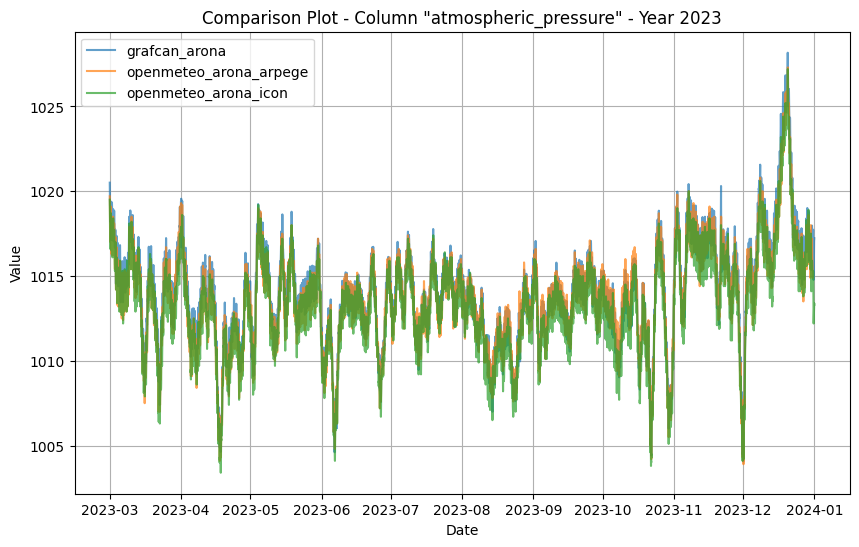
\includegraphics[width=.8\linewidth]{images/visualizacion_1.png}
    \caption{Visualización de la presión atmosférica en Arona durante 2023.}
    \label{visualizacion_1}
\end{figure}
\begin{figure}
    \centering
    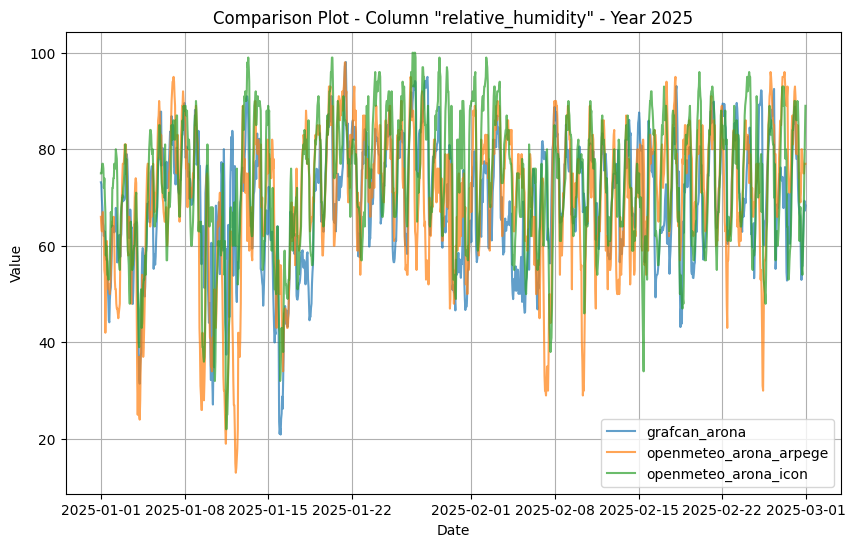
\includegraphics[width=.8\linewidth]{images/visualizacion_2.png}
    \caption{Visualización de la temperatura del aire en Arona durante 2024.}
    \label{visualizacion_2}
\end{figure}
\begin{figure}
    \centering
    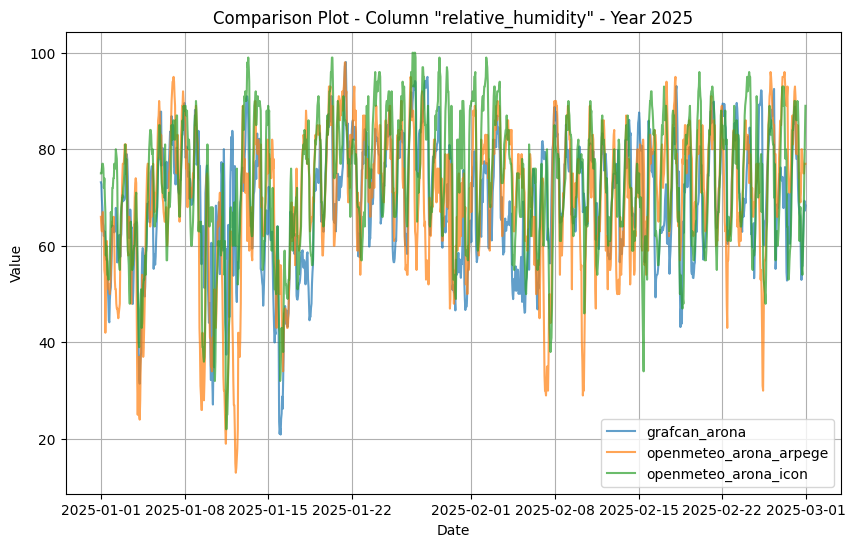
\includegraphics[width=.8\linewidth]{images/visualizacion_3.png}
    \caption{Visualización de la humedad relativa en Arona durante 2025.}
    \label{visualizacion_3}
\end{figure}

Cabe destacar que en la variable de humedad relativa se observa una gran variabilidad entre los datos de las distintas fuentes, que se constatará más adelante.

\subsection{Manejo de datos faltantes}
Se detectan los datos faltantes para cada fuente. Las estadísticas se muestran en la tabla \ref{tabla_datos_faltantes}. 
Es reseñable que el modelo ICON no muestra datos faltantes, mientras que el modelo ARPEGE tiene 35 horas faltantes consecutivas, en el período entre el 31 de diciembre de 2023 y el 1 de enero de 2024.

\begin{table}[htb]
    \small
    \centering
    \begin{tabular}{|c|c|c|c|}
        \hline
        Estación & Grafcan & Open-Meteo ICON & Open-Meteo ARPEGE \\
        \hline
        La Laguna 1 (La Cuesta) & 47 & 0 & 35 \\
        La Laguna 2(La Punta del Hidalgo) & 30 & 0 & 35 \\
        La Orotava & 3 & 0 & 35 \\
        Arona & 17 & 0 & 35 \\
        Garachico & 5 & 0 & 0 \\
        Santa Cruz de Tenerife & 0 & 0 & 46 \\
        \hline
    \end{tabular}
    \caption{Datos faltantes por estación y fuente de datos (en horas)}
    \label{tabla_datos_faltantes} 
\end{table}

Se decide imputar los datos faltantes mediante un método híbrido: si una secuencia de datos faltantes es menor a 5 horas se emplea 
un método de interpolación cúbica por tramos denominado PCHIP\cite{fritsch1980}, que preserva la forma de los datos y evita oscilaciones indeseadas.
Si la secuencia de datos faltantes es mayor a 5 horas, se copian los datos del día anterior en las mismas horas. 
Este tipo de imputación es común en el ámbito de las series temporales \cite{tawakuli2024}.

Los datos sintéticos son etiquetados como tales para poder ser identificados posteriormente.


\subsection{Selección de modelo de Open-Meteo}
Para cada variable se selecciona el modelo de Open-Meteo que mejor se ajusta a los datos de Grafcan.
Se emplean diversas métricas: los coeficiente de correlación de Pearson, Spearman y Kendall, así como el error cuadrático medio (MSE) y 
la distancia euclídea. Se elige el modelo que mejor resultados da en la mayoría de indicadores. Los modelos seleccionados y un ejemplo de las métricas
 se muestran en las tablas \ref{tabla_modelos_seleccionados} y .

\begin{table}[htb]
    \small
    \centering
    \begin{tabular}{|c|c|c|c|}
        \hline
        Estación & Temperatura del aire & Presión atmosférica & Humedad relativa \\
        \hline
        La Laguna 1 & ICON & ARPEGE & ICON \\
        La Laguna 2 & ARPEGE & ARPEGE & ARPEGE \\
        La Orotava & ICON & ARPEGE & ICON \\
        Arona & ICON & ARPEGE & ICON \\
        Garachico & ICON & ICON & ICON \\
        Santa Cruz de Tenerife & ICON & ARPEGE & ICON \\
        \hline
    \end{tabular}
    \caption{Modelo de Open-Meteo seleccionado para cada variable y estación}
    \label{tabla_modelos_seleccionados}
\end{table}

\begin{table}[h!]
\centering
\caption{Métricas de similitud de modelos Open-Meteo con Grafcan para Arona}
\label{tab:sim_metrics}
\footnotesize {
\begin{tabular}{l  cc  cc  cc}
\toprule
\textbf{Métrica} &
\multicolumn{2}{c}{\textbf{air\_temperature}} &
\multicolumn{2}{c}{\textbf{atmospheric\_pressure}} &
\multicolumn{2}{c}{\textbf{relative\_humidity}} \\
\cmidrule(lr){2-3} \cmidrule(lr){4-5} \cmidrule(lr){6-7}
 & \textbf{ICON} & \textbf{ARPEGE} & \textbf{ICON} & \textbf{ARPEGE} & \textbf{ICON} & \textbf{ARPEGE} \\
\midrule
Pearson               & 0.8871 & 0.8415 & 0.9890 & 0.9891 & 0.6281 & 0.3838 \\
Spearman              & 0.9116 & 0.8519 & 0.9859 & 0.9866 & 0.6026 & 0.2748 \\
Kendall               & 0.7489 & 0.6650 & 0.9048 & 0.9070 & 0.4423 & 0.1973 \\
MSE                   & 2.8616 & 5.6179 & 1.1085 & 0.5754 & 208.6453 & 406.1746 \\
Euclidean Distance    & 224.0627 & 313.9447 & 139.4523 & 100.4768 & 1913.2363 & 2669.4431 \\
\bottomrule
\end{tabular}
}
\end{table}


Observamos que, en general, el modelo ICON es el que mejor se ajusta a las variables de temperatura del aire y humedad relativa,
 mientras que el modelo ARPEGE es el que mejor se ajusta a la presión atmosférica.

 Resulta reseñable señalar que la diferencia entre los modelos de Open-Meteo y Grafcan es mucho mayor en la variable 
 de humedad relativa que en las otras. Esto puede ser relevante más adelante, de cara al rendimiento de los modelos de predicción. 

 \bigskip
 Tras selecciona el modelo de Open-Meteo para cada variable, se crea un dataset unificado con las 3 variables. De esta forma se dispone 
 de un dataset de Open-Meteo y otro de Grafcan con las 3 variables para cada estación.

\subsection{Detección de valores anómalos}
Para la detección de valores anómalos, en primer lugar se empea el método del rango intercuartílico (IQR). 
Sin embargo, se observa en los histogramas que la distribución de los datos no es puramente gaussiana, existiendo sesgos y colas largas.
Por ejemplo, en la figura \ref{histogram_1} se observa que la humedad presenta un sesgo a la izquierda, mientras que en la figura 
\ref{histogram_2} se observa que la temperatura presenta una cola larga a la derecha.

\begin{figure}
    \centering
    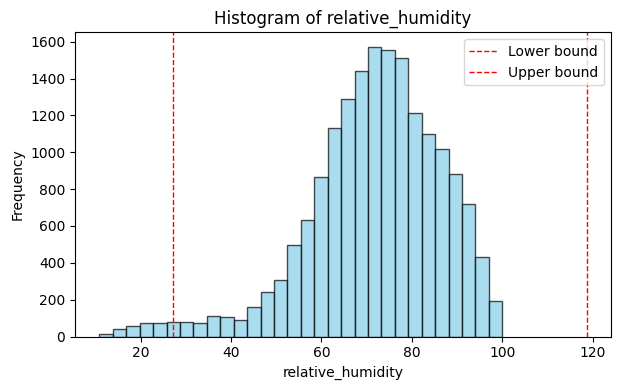
\includegraphics[width=.5\linewidth]{images/histogram_humidity.png}
    \caption{Histograma de la humedad relativa en Arona.}
    \label{histogram_1}
\end{figure}

\begin{figure}
    \centering
    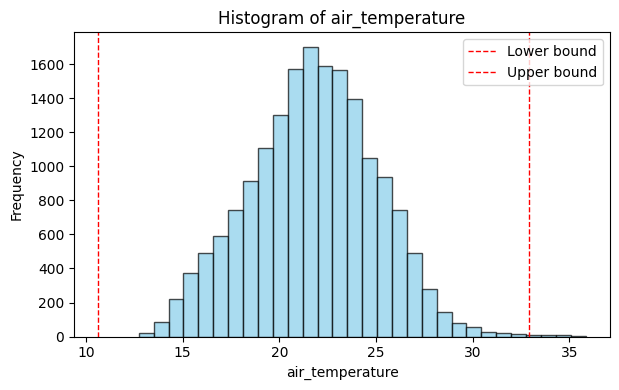
\includegraphics[width=.5\linewidth]{images/histogram_temperature.png}
    \caption{Histograma de la temperatura del aire en Arona.}
    \label{histogram_2}
\end{figure}

Por esto, se decide emplear como método de detección de anomalías el de los K vecinos más cercanos (KNN), 
una alternativa robusta que permite detectar anomalías en distribuciones no gaussianas \cite{gu2019}.

Se aplica el método de KNN a cada variable por separado, con k=10 y límite de distancia 3 veces la desviación típica.
Respecto al número de vecinos (K), se observa al graficar la distancia media de los K vecinos más cercanos frente a K que es poco relevante, por lo que se escoge arbitrariamente.
Una vez fijado K, para determinar el límite se considera que en una distribución gaussiana el 99,7\% de los datos se encuentran dentro de 3 desviaciones típicas y se comprueba empíricamente
este valor, así como otros cercanos, observando los histogramos de los datos detectados como anómalos.

Los valores anómalos son etiquetados como tales para poder ser identificados posteriormente. Se pueden observar ejemplos 
de las distancias en la figura \ref{knn_distances}. En las figuras \ref{histogram_knn_humidity} y \ref{histogram_knn_temperature} se muestran ejemplos de los valores anómalos detectados. 

Nota: Se muestran los valores anómalos indepentientemente de la variable respecto a la que se detectaron.

\begin{figure}
    \centering
    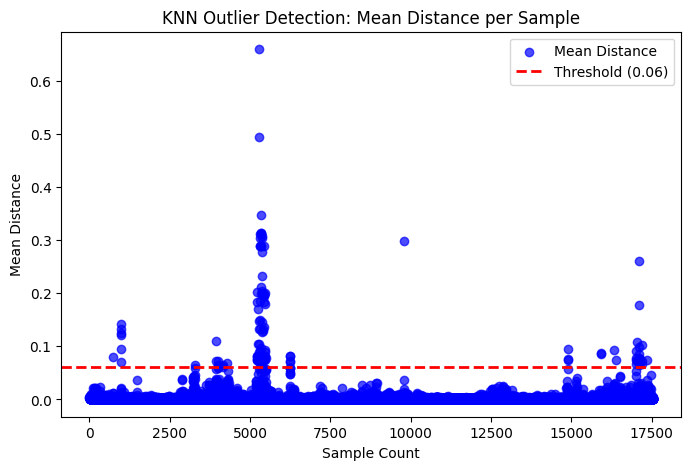
\includegraphics[width=.5\linewidth]{images/knn_distances_temperature_arona.png}
    \caption{Distancias media de los K vecinos más cercanos para la temperatura del aire en Arona.}
    \label{knn_distances}
\end{figure}

\begin{figure}
    \centering
    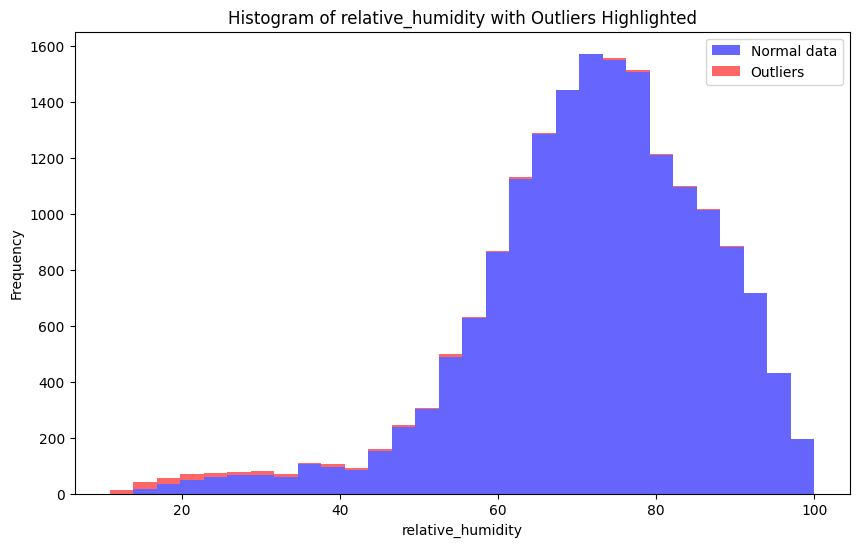
\includegraphics[width=.5\linewidth]{images/histogram_humidity_knn.png}
    \caption{Histograma de la humedad relativa en Arona con outliers detectados con knn.}
    \label{histogram_knn_humidity}
\end{figure}

\begin{figure}
    \centering
    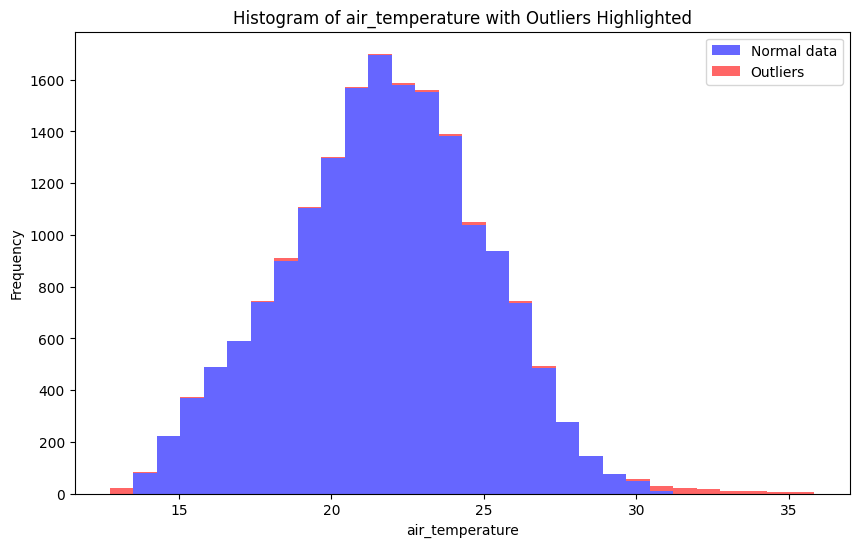
\includegraphics[width=.5\linewidth]{images/histogram_temperature_knn.png}
    \caption{Histograma de la temperatura del aire en Arona con outliers detectados con knn.}
    \label{histogram_knn_temperature}
\end{figure}

\subsection{Exploración de frecuencias - Dominio de Fourier}
Se realiza un análisis de Fourier para cada variable. De esta forma, se pueden observar las frecuencias dominantes en los datos. Este análisis
es relevante para detectar las frecuencias a emplear en la codificación de la información temporal, que se aborda en el siguiente apartado.

Se emplea la transformada rápida de Fourier (FFT), se filtran las frecuencias positivas, se acota a las frecuencias mayores a \(10^{-3}\) 
 (unos 16,66... minutos) y se grafican haciendo uso de escala logarítmica en el eje X. El pseudocódigo se muestra en \ref{fft_positive}. Se pueden observar ejemplos en las figuras \ref{fft_temperature},
 y \ref{fft_pressure}. Se señalan las 5 frecuencias de mayor magnitud con un punto en rojo. 

 \begin{figure}[H]
{\small
 \hrule \
 {\bf\small Pseudocódigo Cálculo de FFT Positiva}
 \hrule
\begin{center}
\begin{tabbing}
\ 1: {\bf Fun}\={\bf ción} calcular\_fft\_positiva($valores$, $intervalo\_muestreo$): \\
\ 2: \> \# 1. Computar la transformada rápida de Fourier del vector de entrada \\
\ 3: \> $fft\_result$ = FFT($valores$)  \\
\ 4: \> \# 2. Generar los intervalos de frecuencia para cada punto de la FFT \\
\ 5: \> $frecuencias$ = FFTFREQ(longitud($valores$), $intervalo\_muestreo$)  \\
\ 6: \> \# 3. Calcular la mitad de la longitud para aislar frecuencias no negativas \\
\ 7: \> $mitad$ = piso(longitud($valores$) / 2)  \\
\ 8: \> \# 4. Extraer solo la parte de frecuencias positivas \\
\ 9: \> $resultado\_fft\_positivo$ = $fft\_result$[0:$mitad$]  \\
\ 10: \> $frecuencias\_positivas$ = $frecuencias$[0:$mitad$]  \\
\ 11: \> \# 5. Calcular la magnitud de los coeficientes complejos resultantes \\
\ 12: \> $magnitud$ = valor\_absoluto($resultado\_fft\_positivo$)  \\
\ 13: \> \# 6. Devolver el eje de frecuencias positivas y su espectro de magnitudes \\
\ 14: \> {\bf Retornar} $frecuencias\_positivas$, $magnitud$  \\
\end{tabbing}
\end{center}
\hrule
}
\caption{Pseudocódigo Cálculo de FFT Positiva}
\label{fft_positive}
\end{figure}


\begin{figure}
    \centering
    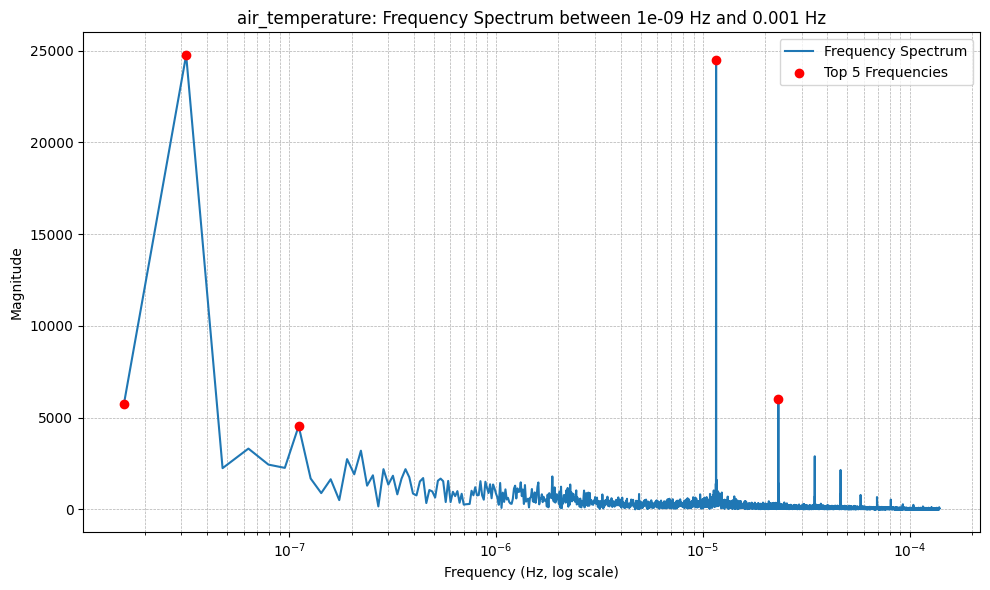
\includegraphics[width=.5\linewidth]{images/fft_temperature.png}
    \caption{Transformada rápida de Fourier de la temperatura del aire en Arona.}
    \label{fft_temperature}
\end{figure}

 \begin{figure}
    \centering
    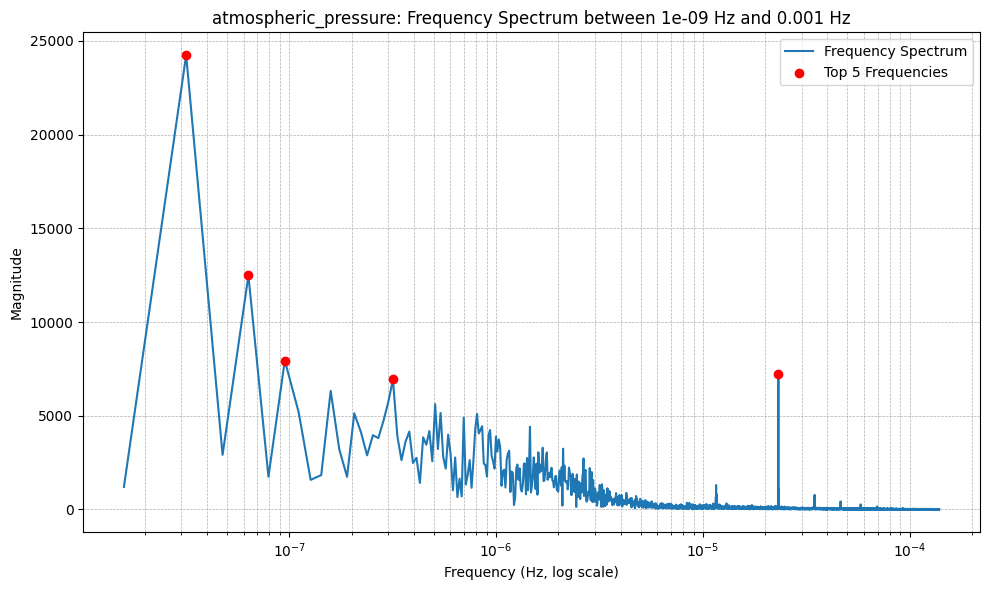
\includegraphics[width=.5\linewidth]{images/fft_pressure.png}
    \caption{Transformada rápida de Fourier de la presión atmosférica en Arona.}
    \label{fft_pressure}
\end{figure}



En la temperatura y humedad destacan las frecuencias de 24 y 8772 horas, correspondiente esta última a 365,5 días, lo que es razonable considerando que de los 
2 años de datos, uno es bisiesto. Respecto a la presión atmosférica, la más relevante es la de 12 horas, algo debido a la naturaleza de esta variable, 
que presenta este ciclo debido a un fenómeno conocido como mareas térmicas \cite{ChapmanLindzen1970}. Así mismo, la presión también presenta un pico en la frecuencia anual y la de medio año.


\subsection{Codificación de la información temporal}
Se decide codificar la información temporal mediante el uso de senos y cosenos de las frecuencias dominantes.
En base a los resultados del análisis de Fourier, se emplean la frecuencia de 24 horas y del año, teniendo especial cuidado para detectar
    si el año es bisiesto o no. De esta forma, se añaden 4 variables adicionales al dataset: sin(dia), cos(diá), sin(año) y cos(año).

Se estudia la frecuencia semanal, pero se descarta al existir poca correlación.

\subsection{Estudio de correlación}
Se estudia la correlación entre las distintas variables que conforman el dataset mediante una matriz de correlación con el coeficiente de Pearson.
Se observa que las variables climáticas tienen una correlación negativa de en torno a 0.3, lo que indica que las variables están relacionadas de 
forma baja/moderada e inversamente proporcional \ref{correlation_map}.

\begin{figure}
    \centering
    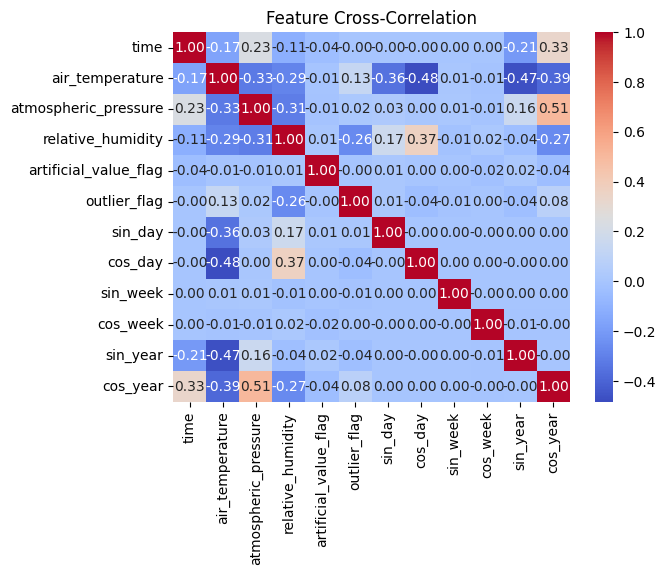
\includegraphics[width=.5\linewidth]{images/correlation_heatmap.png}
    \caption{Mapa de correlación entre las variables del dataset.}
    \label{correlation_map}
\end{figure}

\section{Creación de ventanas de datos}
Para la predicción de series temporales, los modelos neuronales requieren como entrada los valores de las variables en un número de instantes, en nuestro caso horas,
previos, que denominaremos P. Así mismo, se define un número de horas a predecir, que denominaremos N. 
De esta forma, un modelo requiere P horas de datos para predecir N horas futuras. Esto es lo que se conoce como ventana de datos.

En su versión más simple, la univariable, consta de una componente X, los valores de la variable en P pasos, y una componente Y, un vector
de tamaño N con los valores a predecir. 
No obstante, puede ser relevante incluir información adicional exógena sobre los valores a predecir, como la codificación temporal 
(o en otros dominios, si el día es festivo, etc).

Optamos por incluir esta información y contruir ventanas de datos con 3 componentes, X e Y, ya definidas, así como F, formada por las 4 variables de codificación temporal 
para cada paso a predecir N. Empíricamente comprobamos que la inclusión de esta información adicional mejora ligeramente el rendimiento del modelo.

En la práctica, estas ventanas se construyen mediante la técnica de ventana deslizante, que consiste en recorrer la serie temporal desplazando 
la ventana de datos en un número de pasos, que denominaremos S. Establecemos S=6 para que la ventana se desplace cada 6 horas, con el fin de buscar un balance 
entre evitar la redundancia de datos que existiría si usásemos un paso menor y mantener el máximo de información posible.

Como datos pasados empleamos la variable meteorológcia estudiada, así como las restantes como covariables. Se comprueba empíricamente que 
añadir estas covariables mejora el rendimiento del modelo. También se emplea como datos pasados las variables de codificación temporal. 

Es decir, la estructura de una ventana es:
\itemize{
    \item X: un vector de tamaño P * 7, que contiene los valores de la variable objetivo y las covariables en los pasos previos.
    \item F: un vector de tamaño N * 4, que contiene las variables de codificación temporal para cada paso a predecir.
    \item Y: un vector de tamaño N, que contiene los valores a predecir.
}

\subsection{Implementación}
En primer lugar, se define una función \textit{df\_raw\_windows} que recibe como parámetros:
\itemize{
    \item df: un dataframe de pandas, que es una estructura de datos de python similar a una tabla, correspondiente a un dataset de una ubicación,
    \item P: el número de pasos pasados.
    \item N: el número de pasos a predecir.
    \item S: el número de pasos a desplazar la ventana.
    \item past\_features: un array con los nombres de las variables usadas como entradas.
    \item future\_features: un array con los nombres de las variables exógenas usadas como datos futuros.
    \item target: el nombre de la variable objetivo a predecir.
}

La función devuelve un objeto con 3 atributos,\textit{past\_variables}, \textit{future\_variables} e \textit{y}.
Siendo cada uno un arreglo con los datos de cada componente de las ventanas de datos. Es decir, la ventana i ésima
está formada por los iésimos elementos de cada uno de los 3 atributos. Esta estructura se debe al comportamiento
de las librerías de los modelos de aprendizaje profundo empleados, que procesan los datos de forma más eficiente en este formato,
como se verá más adelante.

\bigskip
El comportamiento de la función principal es el siguiente:

\begin{figure}[H]
{\small
 \hrule \
 {\bf\small Pseudocódigo Creación de Ventanas de Datos}
 \hrule
\begin{center}
\begin{tabbing}
\ 1: $train\_data$ = \{\} \\
\ 2: $test\_data$ = \{\} \\
\ 3: {\bf Par}\={\bf a cada} variable objetivo $v$: \\
\ 4: \> {\bf Par}\={\bf a cada} ubicación $u$:  \\
\ 5: \> $location\_data$ = [] \\
\ 6: \> \> {\bf Par}\={\bf a cada} dataset $d$ en la ubicación $u$:  \\
\ 7: \> \> \> $ventanas$ =  \textit{df\_raw\_windows()} \\
\ 8: \> \> \> $location\_data$.añadir($ventanas$) \\
\ 9: \> \> $windows\_count$ = len($location\_data$[0][$y$]) \\
\ 10: \> \> $overlap\_windows$ = ceil(($past\_n$ + $future\_n$)/$step$) \\
\ 11: \> \> $test\_indexes$ = random\_sample($windows\_count$, $test\_percent$) \\
\ 12: \> \> $forbidden$ = set() \\
\ 13: \> \> {\bf Par}\={\bf a cada} $index$ en $test\_indexes$: \\
\     \> \> \>   \# Prohibir el índice y las siguientes `$overlap\_windows$ - 1` ventanas \\
\ 14: \> \> \>   {\bf Par}\={\bf a cada} \= $j$ en rango($overlap\_windows$): \\
\ 15: \> \> \> \>     $forbidden$.add($index$ + $j$) \\
\ 16: \> \> $train\_indexes$ = rango($windows\_count$) - $forbidden$ \\

\ 17: \> \> {\bf Par}\={\bf a cada} dataset $d$ en $location\_data$: \\
\ 18: \> \> \> $past\_variables\_windows$ = $location\_data$[$d$]["past\_variables"] \\
\ 19: \> \> \> $future\_variables\_windows$ = $location\_data$[$d$]["future\_variables"] \\
\ 20: \> \> \> $y\_windows$ = $location\_data$[$d$]["y"] \\
\     \> \> \> \# Construcción de conjuntos de entrenamiento y validación \\
\ 21: \> \> \> $train\_past\_variables$ = [$past\_variables\_windows$[i] para i en $train\_indexes$] \\
\ 22: \> \> \> $train\_future\_variables$ = [$future\_variables\_windows$[i] para i en $train\_indexes$] \\
\ 23: \> \> \> $train\_y$ = [$y\_windows$[i] para i en $train\_indexes$] \\

\ 24: \> \> \> $test\_past\_variables$ = [$past\_variables\_windows$[i] para i en $test\_indexes$] \\
\ 25: \> \> \> $test\_future\_variables$ = [$future\_variables\_windows$[i] para i en $test\_indexes$] \\
\ 26: \> \> \> $test\_y$ = [$y\_windows$[i] para i en $test\_indexes$] \\
      
\ 27: \> \> \> $train\_data$[$v$]["past\_variables"].extender($train\_past\_variables$) \\
\ 28: \> \> \> $train\_data$[$v$]["future\_variables"].extender($train\_future\_variables$) \\
\ 29: \> \> \> $train\_data$[$v$][\string"y"].extender($train\_y$) \\
        
\ 30: \> \> \> $test\_data$[$v$]["past\_variables"].extender($test\_past\_variables$) \\
\ 31: \> \> \> $test\_data$[$v$]["future\_variables"].extender($test\_future\_variables$) \\
\ 32: \> \> \> $test\_data$[$v$][\string"y"].extender($test\_y$) \\

\end{tabbing}
\end{center}
\hrule
}
\caption{Pseudocódigo Creación de Ventanas de Datos}
\label{branch_and_bound_max_diversity}
\end{figure}

La construcción del conjunto de entrenamiento y test se realiza de forma aleatoria, algo poco común en el ámbito de la predicción de series temporales, puesto que habitualmente 
se emplea como conjunto de validación un período al final de la serie. Pero, de esta forma, creemos que se puede mejorar el modelo, al disponer de un conjunto de validación
más diverso y representativo de la meteorología a lo largo del año.

Para cada ubicación se eligen los índices de las ventanas de test aleatoriamente. Estos índices son los mismos para los dos datasets de una localización, 
puesto que los datos son bastante similares entre ambos y queremos evitar el filtrado de información. 
Cabe destacar la consideración de ventanas "prohibidas", que se descartan del conjunto de entrenamietno para evitar filtrar datos.
De esta forma, todas las ventanas previas que estén solapadas con una ventana de test son descartadas.

De todas las ventanas creadas originalmente, se escogen un 10\% para el conjunto de test. Como se descartan las ventanas solapadas, según los parámetros empleados, la división resultantes
es de alrededor de un 14\% de ventanas de test y un 86\% de ventanas de entrenamiento. Se eligen estos porcentajes puesto que se comprueba empíricamente que a un mayor número de 
ventanas de entrenamiento el rendiemiento del modelo mejora, pero se fija el límite del 10\% para conseguir un conjunto de test representativo y diverso. Esto supone unas 2.300 ventanas
de validación y entre 13.900 y 12.500 de entrenamiento según las características de la ventana elegidas. 

\subsection{Normalización}
Se utilizan las ventanas del conjunto de entremaniento para calcular las características de la normalización.
Usamos la estandarización o normalización Z-score, que consiste en restar la media y dividir por la desviación típica.
De esta forma, los datos quedan centrados en 0 y con una desviación típica de 1.

La normalización se aplica a la variable objetivo y las covariables meteorológicas, tanto en los datos pasados como los datos a predecir ($y$). 
No se aplica a las variables de codificación temporal, ya que al tratarse de senos y cosenos, su rango ya es limitado entre -1 y 1.

Debemos almacenar los parámetros de normalización puesto que serán necesarios para tratar cualquier dato que se suministre en el futuro al sistema.


%%%%%%%%%%%%%%%%%%%%%%%%%%%%%%%%%%%%%%%%%%%%%%%%%%%%%%%%%%%%%%%%%%%%%%%%%%%%%%%
\newpage{\pagestyle{empty}}
\thispagestyle{empty}

\chapter{\LARGE Modelos de predicción}
\label{chapter:tres}

Se desarrollan 4 modelos: un modelo ARIMA como base de comparación, un modelo LSTM, un modelo CNN y un híbrido LSTM-CNN.

\section{ARIMA}
Los modelos ARIMA (Autoregressive Integrated Moving Average) son un tipo de modelos estadísticos utilizados históricamente para el análisis y la predicción de series temporales
univariable. 

Utilizamos como base de comparación los resultados de un ARIMA para cada serie temporal: cada variable en cada ubicación y cada fuente de datos.

Para emplear un modelo ARIMA, es necesario ajustar cada uno de sus parámetros, que son:
\begin{itemize}
    \item $p$: el número de términos autorregresivos (AR).
    \item $d$: el número de diferencias necesarias para hacer la serie estacionaria (I).
    \item $q$: el número de términos de media móvil (MA).
\end{itemize}

\subsection{Calibración de términos autorregresivos}
Para determinar el número de términos autorregresivos, se utiliza la función \texttt{plot\_pacf} de la librería \texttt{statsmodels}, 
que permite visualizar la función de autocorrelación parcial (PACF) de la serie temporal. Observamos ejemplos de los resultados en las figuras \ref{arima_pacf_hum}, \ref{arima_pacf_pres}. 

\begin{figure}[H]
    \centering
    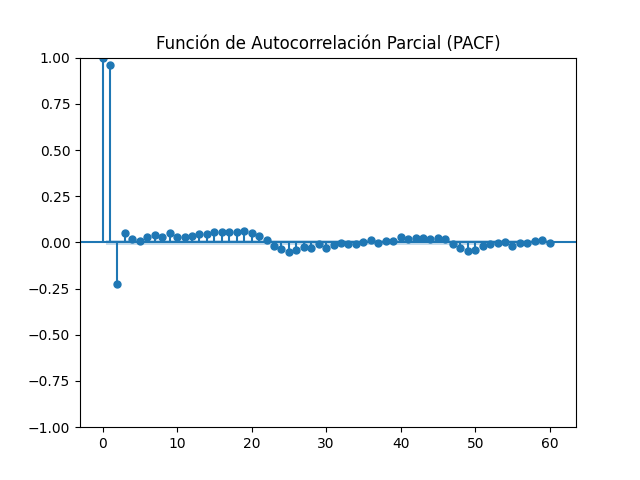
\includegraphics[width=0.5\textwidth]{images/arima_pacf_hum.png}
    \caption{Gráfico de PACF para la serie de humedad relativa en La Laguna de GRAFCAN}
    \label{arima_pacf_hum}
\end{figure}

\begin{figure}[H]
    \centering
    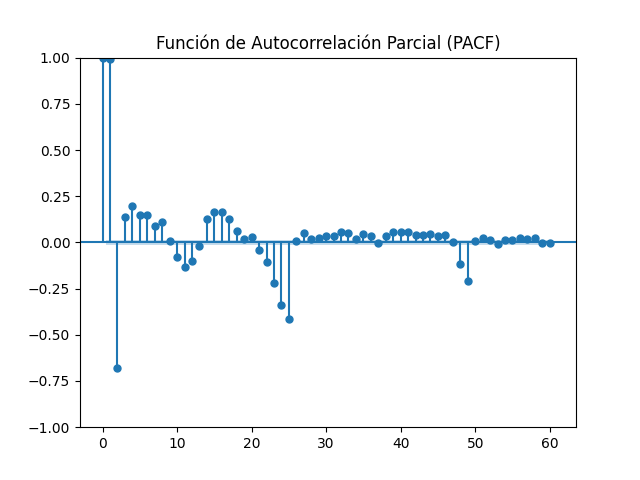
\includegraphics[width=0.5\textwidth]{images/arima_pacf_pres.png}
    \caption{Gráfico de PACF para la serie de presión atmosférica en La Laguna de GRAFCAN}
    \label{arima_pacf_pres}
\end{figure}


Analíticamente, se emplea el algoritmo descrito en \ref{pacf_ar_order}. Se determina $p$ = 4 para las series de temperatura del aire y humedad relativa, mientras 
que se obtiene $p$ = 8 en el caso de la presión atmosférica.

\begin{figure}[H]
    {\small
    \hrule \
    {\bf\small Pseudocódigo Selección de Orden AR vía PACF}
    \hrule
    \begin{center}
    \begin{tabbing}
    \ 1: {\bf Fun}\={\bf ción} seleccionar\_orden\_AR($serie$, $max\_lags$): \\
    \ 2: \> \# 1. Calcular la PACF hasta $max\_lags$ retardos \\
    \ 3: \> $pacf\_valores$ = PACF($serie$, $nlags$=$max\_lags$) \\
    \ 4: \> \# 2. Definir intervalo de confianza al 95\% \\
    \ 5: \> $intervalo\_confianza$ = 1.96 / raiz\_cuadrada(longitud($serie$)) \\
    \ 6: \> \# 3. Buscar el primer retardo no significativo \\
    \ 7: \> {\bf Para} \= $lag$ {\bf en} 1 \dots $max\_lags$: \\
    \ 8: \> \> {\bf Si} \= valor\_absoluto($pacf\_valores[lag]$) $<$ $intervalo\_confianza$: \\
    \ 9: \> \> \> imprimir("El mejor orden AR sugerido por la PACF es:", $lag-1$) \\
    \ 10: \> \> \> {\bf Retornar} $lag-1$ \\
    \ 11: \> \# 4. Si todos los retardos son significativos \\
    \ 12: \> imprimir("Todos los retardos hasta", $max\_lags$, "son significativos.) \\
    \ 13: \> {\bf Retornar} $max\_lags$ \\
    \end{tabbing}
    \end{center}
    \hrule
    }
    \caption{Pseudocódigo para Selección de Orden AR usando PACF}
    \label{pacf_ar_order}
\end{figure}

\subsection{Estudio de la estacionariedad}
Se emplea la prueba de Dickey-Fuller aumentada (ADF) para determinar la estacionariedad de las series temporales.
La prueba ADF es una prueba estadística que evalúa la presencia de una raíz unitaria en una serie temporal, lo que indica si la serie es estacionaria o no.
La hipótesis nula de la prueba ADF establece que la serie temporal tiene una raíz unitaria, lo que implica que no es estacionaria.
Si el valor p de la prueba es menor que un nivel de significancia predefinido (por ejemplo, 0.05), se rechaza la hipótesis nula y se concluye que la serie es estacionaria.

Empleamos como significancia un nivel de 0.05, y se observa que todas las series temporales son estacionarias, por lo que no es necesario aplicar diferencias, 
es decir, $d$ = 0.

\subsection{Determinación del orden de la media móvil}
Para calcular el número de términos de media móvil, se utiliza la función de Autocorrelación \texttt{ACF} de la librería \texttt{statsmodels}. Dicha función 
retorna los coeficientes de autocorrelación para diferentes retardos.

Analíticamente, se emplea el algoritmo descrito en \ref{acf_ma_order}, cuya idea principal consiste en comprobar para cada retardo si el 
coeficiente de autocorrelación es significativo, finalizando cuando se encuentra el primer retardo no significativo. 

Se calcula el intervalo de confianza como 1.96 por la raíz cuadrada de la longitud de la serie temporal, ya que la distribución de
la autocorrelación estimada en cualquier lag se aproxima a una distribución normal con media 0 y desviación estándar $\frac{1}{\sqrt{n}}$,
donde $n$ es el número de observaciones. De esta forma se obtiene un intervalo de confianza al 95\% para la autocorrelación. No obstante, se establece 
un límite inferior de 0.05 para evitar que el nivel de significancia sea demasiado bajo y se detecte el ruido como una señal significativa.
\begin{figure}[H]
    {\small
    \hrule \
    {\bf\small Pseudocódigo Selección de Orden MA vía ACF}
    \hrule
    \begin{center}
    \begin{tabbing}
    \ 1: {\bf Fun}\={\bf ción} seleccionar\_orden\_MA($serie$, $max\_lags$, $min\_confidence$): \\
    \ 2: \> \# 1. Calcular la ACF hasta $max\_lags$ retardos \\
    \ 3: \> $acf\_valores$ = ACF($serie$, $nlags$=$max\_lags$) \\
    \ 4: \> \# 2. Definir intervalo de confianza al 95\% \\
    \ 5: \> $intervalo\_confianza$ = max(1.96 / raiz\_cuadrada(longitud($serie$)), $min\_confidence$) \\
    \ 6: \> \# 3. Buscar el primer retardo no significativo \\
    \ 7: \> {\bf Para} \= $lag$ {\bf en} 1 \dots $max\_lags$: \\
    \ 8: \> \> {\bf Si} \= valor\_absoluto($acf\_valores[lag]$) $<$ $intervalo\_confianza$: \\
    \ 9: \> \> \> imprimir("El mejor orden MA sugerido por la ACF es:", $lag-1$)\\
    \ 10: \> \> {\bf Retornar} $lag-1$\\
    \ 11: \> {\bf Retornar} $max\_lags$\\
    \end{tabbing}
    \end{center}
    }
    \hrule
    \caption{Pseudocódigo para Selección de Orden MA usando ACF}
    \label{acf_ma_order}
\end{figure}

El algoritmo descrito retorna el máximo número de retardos para valores elevados de lags, por lo que se analiza el gráfico de la ACF y se observa que
no existe un punto de corte claro, sino que existe un descenso suave y progresivo para todas las variables \ref{acf_arima_temp} \ref{acf_arima_pres}. Por lo tanto, se fija $q$ = 0.

\begin{figure}[H]
    \centering
    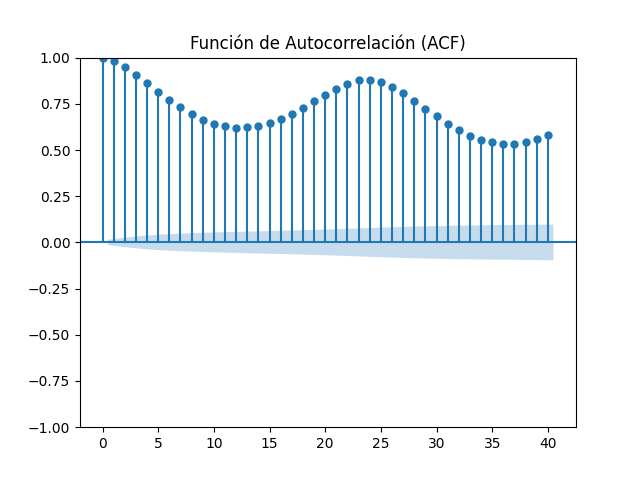
\includegraphics[width=0.5\textwidth]{images/arima_acf_temp.png}
    \caption{Gráfico de ACF para la serie de temperatura del aire en La Laguna de GRAFCAN}
    \label{acf_arima_temp}
\end{figure}

\begin{figure}[H]
    \centering
    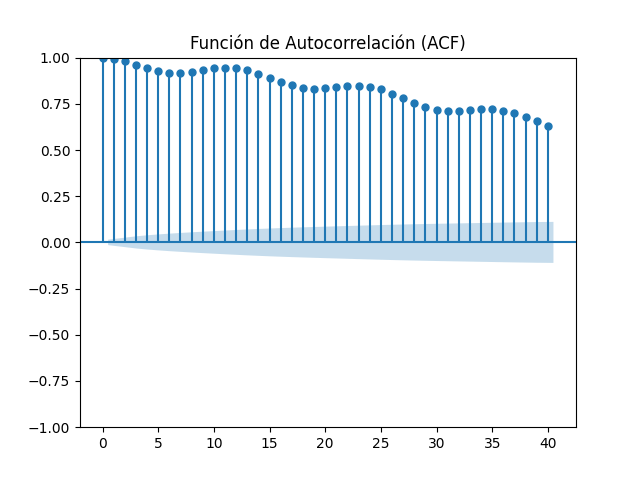
\includegraphics[width=0.5\textwidth]{images/arima_acf_pres.png}
    \caption{Gráfico de ACF para la serie de presión atmosférica en La Laguna de GRAFCAN}
    \label{acf_arima_pres}
\end{figure}

\subsection{Evaluación}
Para evaluar los modelos ARIMA empleamos la validación progresiva (walk-forward validation), que consiste en un bucle en el que se entrena al modelo, se realiza una predicción y se reentrena con los datos más recientes
antes de realizar la siguiente predicción. Este proceso se repite hasta que se alcanza el final del periodo de validación \ref{walk_forward_arima}. Emplearemos como métrica la raíz del error cuadrático medio (RMSE), 
que se calcula como la raíz cuadrada de la media de los errores al cuadrado entre las predicciones y los valores reales. Esta medición proporciona el error en la unidad de la variable.

\begin{figure}[H]
{\small
\hrule
{\bf\small Pseudocódigo Validación Walk-Forward con ARIMA}
\hrule
\begin{center}
\begin{tabbing}
\ 1: {\bf Fun}\={\bf ción} validacion\_walk\_forward($test$, $history$, $pasos\_prediccion$, $orden\_ARIMA$): \\
\ 2: \> $predicciones$ = lista\_vacía() \\
\ 3: \> $valores\_reales$ = lista\_vacía() \\
\ 4: \> {\bf Para} \= $t$ {\bf en} rango(0, longitud($test$) $-$ $pasos\_prediccion$ $+$ 1, $pasos\_prediccion$): \\
\ 5: \> \> $modelo$ = ARIMA($history$, orden=$orden\_ARIMA$) \\
\ 6: \> \> $ajuste$ = ajustar($modelo$) \\
\ 7: \> \> $pronostico$ = predecir($ajuste$, pasos=$pasos\_prediccion$) \\
\ 8: \> \> $predicciones$.añadir($pronostico$) \\
\ 9: \> \> $valores\_reales$.añadir($test[t : t+pasos]$) \\
\ 10: \> \> $history$.añadir($test[t : t+pasos]$) \\
\ 11: \> $rmse$ = raíz\_cuadrada(ECM($valores\_reales$, $predicciones$)) \\
\ 12: \> {\bf Retornar} $rmse$ \\
\end{tabbing}
\end{center}
}
\hrule
\caption{Pseudocódigo para validación walk-forward usando ARIMA}
\label{walk_forward_arima}
\end{figure}

Se toma como ejemplo la serie de temperatura del aire en Arona de Open-Meteo, con un horizonte de predicción de 3 horas. En la figura \ref{arima_residuals} se observan los residuos (diferencia entre valor real y predicción), mientras que en \ref{arima_residuals_density} se observa la estimación de la distribución de la densidad de los residuos.
Al estar centrada en 0 y tener una forma similar a la campana de Gauss, se puede concluir que el modelo ARIMA se ajusta bien a los datos. Finalmente, en la figura 
\ref{arima_results_graph} se muestra un ejemplo de los resultados obtenidos.

\begin{figure}
    \centering
    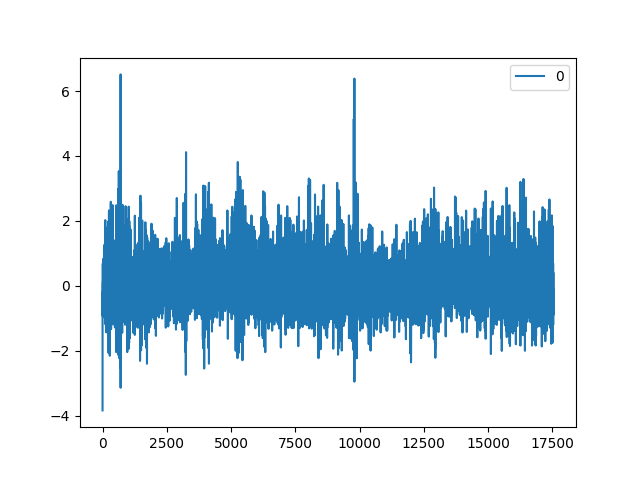
\includegraphics[width=0.7\textwidth]{images/arima_residuals.png}
    \caption{Residuos del modelo ARIMA para la serie de temperatura del aire en Arona de Open-Meteo}
    \label{arima_residuals}
\end{figure}

\begin{figure}
    \centering
    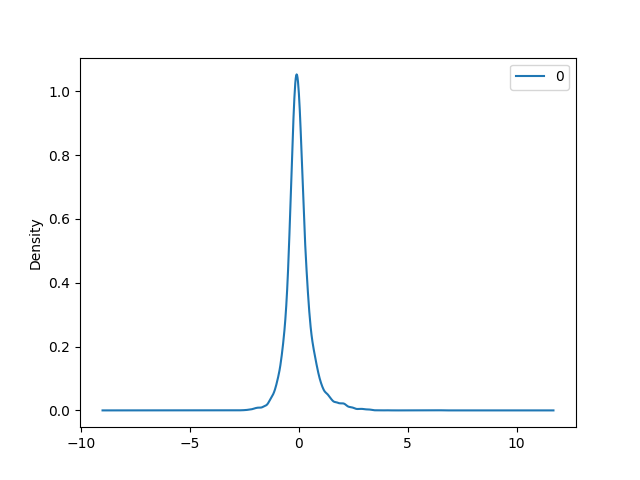
\includegraphics[width=0.7\textwidth]{images/arima_residuals_density.png}
    \caption{Distribución de los residuos del modelo ARIMA para la serie de temperatura del aire en Arona de Open-Meteo}
    \label{arima_residuals_density}
\end{figure}

\begin{figure}[H]
    \centering
    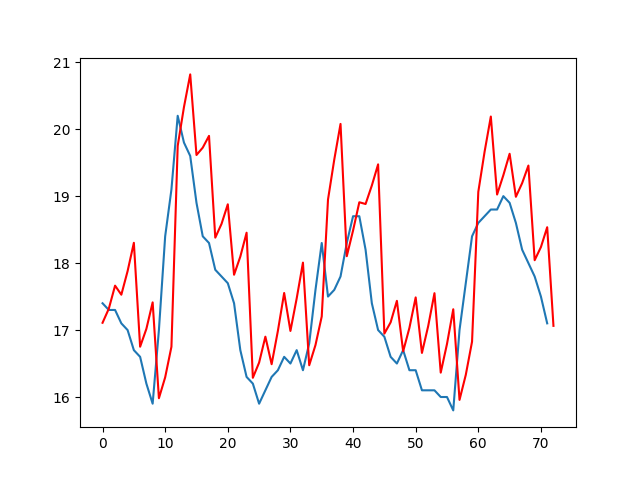
\includegraphics[width=0.7\textwidth]{images/arima_result.png}
    \caption{Resultados del modelo ARIMA para la serie de temperatura del aire en Arona de Open-Meteo}
    \label{arima_results_graph}
\end{figure}

\section{Modelos de aprendizaje profundo}
Existen diferentes frameworks para el desarrollo de modelos de aprendizaje profundo, destacando TensorFlow, PyTorch o JAX/Flax como los más extendidos.
Después de evaluar alternativas, se opta por TensorFlow debido a su amplia comunidad de usuarios y su extensa documentación, así como por su integración con Keras, 
una biblioteca de alto nivel que facilita la creación de modelos de aprendizaje profundo.

\subsection{Creación del dataset con TensorFlow}
Para crear el dataset, se emplea la función de TensorFlow \texttt{Dataset.from\_tensor\_slices()}, que permite crear un objeto Dataset 
a partir de tensores de entrada y salida. Dichos tensores son: la dupla (datos\_pasados, datos\_futuros) y el arreglo con los datos de validación.

Se crean dos datasets: uno para el entrenamiento y otro para la validación. Ambos se dividen en lotes (batches) de tamaño 64. Este número se elige tras realizar 
pruebas con diferentes tamaños de lotes en los distintos modelos, y se observa que, pese a ser un poco más inestable, ya que un número pequeño de muestras por lote
puede causar que el modelo cambie de forma exagerada en algún lote, con ese valor se consiguen los modelos con menor error. 

En el caso del conjunto de entrenamiento, tras crear los lotes se baraja, para evitar el sobreajuste y mejorar la generalización del modelo.

\subsection{Consideraciones generales}
Se emplea como métrica de pérdida el error mse de las ventanas de validación.

Además, para controlar el entrenamiento se emplean dos funciones de retorno (callbacks): 
\begin{itemize}
\item \texttt{EarlyStopping}: detiene el entrenamiento si no se observa mejora en la métrica de validación durante un número determinado de épocas (patience). 
De esta forma se intenta evitar el sobreajuste. Además, se guarda el modelo con la mejor métrica de validación.
\item \texttt{ReduceLORonPlateau}: reduce la tasa de aprendizaje por un factor si no se observa mejora en la métrica de validación durante un número determinado de épocas (patience).
Se basa en la idea de que cuando el modelo no mejora, es posible que se encuentre cerca de un mínimo local y que una tasa de aprendizaje más baja pueda ayudar a acercarse más.
\end{itemize}

Para determinar estas variables, además de otros hiperparámetros como el ratio de aprendizaje, se hace uso de una herramienta de ajuste fino (fine-tuning). En particular, se emplea Keras Tuner, y el método de búsqueda
en rejilla (grid search), que consiste en definir un espacio de búsqueda para los hiperparámetros y evaluar todas las combinaciones posibles. Se realizan 5 ejecuciones por prueba y se 
emplea la media de los resultados.

\subsection{CNN}
Las redes convolucionales (CNN) son un tipo de red neuronal diseñada originalmente para procesar datos con estructura de cuadrícula (como imágenes), pero también se pueden aplicar a series temporales (1D).
Su base es la convolución, una operación en la que uno o varios filtros (o núcleos) se deslizan sobre la entrada, calculando productos escalares para extraer características locales relevantes.
Cada filtro tiene un tamaño (kernel size) y avanza con un paso (stride) determinado; además, puede aplicarse padding (relleno) para controlar las dimensiones de la salida.
En una capa suelen existir múltiples filtros distintos, de manera que cada uno aprende a detectar un patrón diferente (por ejemplo, tendencias, picos o frecuencias concretas en series temporales).

Tras las capas convolucionales, es común intercalar capas de pooling (submuestreo), como max-pooling o average-pooling, para reducir dimensión, extraer características más robustas y controlar el sobreajuste.
Durante el entrenamiento de la red, los pesos de los filtros se ajustan para minimizar el error de predicción.

Se muestra el pseudocódigo del modelo CNN desarrollado para este trabajo en la figura \ref{cnn_model}. Se descarta el uso de pooling tras estudiar varias alternativas, ya que no se observa mejora en 
el rendimiento del modelo. También se contempla el uso de múltiples capas de convolución, tanto en el flujo de datos pasado, como en el futuro o después de concatenarlo, así como apiladas. 
Sin embargo, el mejor modelo es el que se muestra, con una sola capa de convolución en los datos pasados, una capa densa para los futuros y otra densa para la salida.
Cabe destacar el uso de relleno o padding de tipo causal que evita que la red vea datos futuros al realizar la convolución, lo que es especialmente importante en series temporales, puesto que es 
importante que la red no tenga acceso a información futura y entienda la causalidad.

\begin{figure}[H]
{\small
\hrule
{\bf\small Pseudocódigo para el modelo CNN}
\hrule
\begin{center}
\begin{tabbing}
\ 1: {\bf Fun}\={\bf ción construir\_modelo}($past\_data\_shape$, \\
\  \> $future\_data\_shape$, $forecast\_length$, $learning\_rate$): \\
\ 3: \> $entrada\_pasado$ = Input(shape=$past\_data\_shape$) \\
\ 4: \> $entrada\_futuro$ = Input(shape=$future\_data\_shape$) \\
\ 5: \> \# Procesar datos pasados con una capa convolucional y flatten \\
\ 6: \> $x1$ = Conv1D(filtros=42, kernel=3, activación='ReLU', padding='causal')($entrada\_pasado$) \\
\ 7: \> $x1$ = Flatten()($x1$) \\
\ 8: \> \# Procesar datos futuros con flatten y capa densa \\
\ 9: \> $x2$ = Flatten()($entrada\_futuro$) \\
10: \> $x2$ = Dense(unidades=4, activación='ReLU')($x2$) \\
11: \> \# Combinar representaciones \\
12: \> $y$ = concatenar($x1$, $x2$) \\
13: \> $salida$ = Dense(unidades=$forecast\_length$)($y$) \\
14: \> \# Construir y compilar el modelo \\
15: \> modelo = Modelo(entradas=[ $entrada\_pasado$, $entrada\_futuro$ ], salidas=$salida$) \\
16: \> compilar(modelo, optimizador=Adam($learning\_rate$), pérdida='MSE') \\
17: \> {\bf Retornar} modelo \\
\end{tabbing}
\end{center}
}
\hrule
\caption{Pseudocódigo del modelo CNN}
\label{cnn_model}
\end{figure}


\subsection{LSTM}
Las redes LSTM (Long Short-Term Memory) son un tipo de red neuronal recurrente (RNN) que se utilizan para modelar secuencias temporales.
Las LSTM son capaces de aprender patrones a largo plazo en los datos, lo que las hace adecuadas para tareas de predicción de series temporales.
Se basan en la idea de utilizar celdas de memoria que pueden almacenar información durante períodos prolongados, lo que les permite recordar información relevante de entradas anteriores.
Cada unidad LSTM incluye una celda de memoria y tres puertas que regulan el flujo de información:
\begin{itemize}
\item Puerta de entrada: decide qué información nueva se añade a la celda de memoria.
\item Puerta de olvido: determina qué información de la celda de memoria se olvida.
\item  Puerta de salida: controla qué información de la celda de memoria se envía como salida.
\end{itemize}

Son relevantes también las capas bidireccionales. Introducidas en 2005 por Graves y Schmidhuber \cite{graves_schmidhuber2005}, las LSTM bidireccionales permiten que la red procese la secuencia de 
entrada en ambas direcciones (hacia adelante y hacia atrás), lo que mejora la capacidad de capturar dependencias a largo plazo en los datos, ayudando, por ejemplo, a evitar
ambigüedades debido al mayor contexto.

La estructura de los modelos LSTM desarrollados puede observarse en el apartado \ref{sec:resultados}. 

\subsection{Híbrido LSTM-CNN}
Los modelos híbridos LSTM-CNN combinan las ventajas de las redes LSTM y las redes convolucionales. Intercalan capas convolucionales y LSTM para capturar tanto patrones locales como dependencias a largo plazo en los datos de series temporales.
La arquitectura típica de un modelo LSTM-CNN incluye capas convolucionales iniciales para extraer características locales, seguidas de capas LSTM para capturar patrones temporales a largo plazo.

Se desarrolla un modelo híbrido estudiando distintas combinaciones de capas LSTM y convolucionales, decidiendose por una capa convolucional seguida de una LSTM bidireccional para los datos pasados,
una capa densa para los datos futuros y una capa densa para la salida. El modelo se describe en la figura \ref{cnn_bilstm_model}.

\begin{figure}[H]
{\small
\hrule
{\bf\small Pseudocódigo para el modelo híbrido CNN + BiLSTM}
\hrule
\begin{center}
\begin{tabbing}
\ 1: {\bf Fun}\= {\bf ción construir\_modelo}($past\_data\_shape$, $future\_data\_shape$,$forecast\_length$, $learning\_rate$): \\
\ 2: \> \# Definir capas de entrada \\
\ 3: \> $entrada\_pasado$ = Input(shape=$past\_data\_shape$) \\
\ 4: \> $entrada\_futuro$ = Input(shape=$future\_data\_shape$) \\
\ 5: \> \# Procesar datos pasados con Conv1D y BiLSTM \\
\ 6: \> $past$ = Conv1D(filtros=42, kernel=2, activación='ReLU', padding='causal')($entrada\_pasado$) \\
\ 7: \> $past$ = BiLSTM(unidades=42, return\_sequences=False)($past$) \\
\ 8: \> \# Procesar datos futuros con Flatten y Dense \\
\ 9: \> $decoder\_lstm$ = Flatten()($entrada\_futuro$) \\
10: \> $decoder\_lstm$ = Dense(unidades=4, activación='ReLU')($decoder\_lstm$) \\
11: \> \# Combinar representaciones \\
12: \> $merged$ = concatenar($past$, $decoder\_lstm$) \\
13: \> $salida$ = Dense(unidades=$forecast\_length$)($merged$) \\
14: \> \# Construir y compilar el modelo \\
15: \> modelo = Modelo(entradas=[ $entrada\_pasado$, $entrada\_futuro$ ], salidas=$salida$) \\
16: \> compilar(modelo, optimizador=Adam($learning\_rate$), pérdida='MSE') \\
17: \> {\bf Retornar} modelo \\
\end{tabbing}
\end{center}
}
\hrule
\caption{Pseudocódigo del modelo Híbrido CNN + BiLSTM}
\label{cnn_bilstm_model}
\end{figure}


\section{Comparativa inicial}
Para establecer una referencia del rendimiento de los modelos neuronales, se compara un modelo LSTM con un modelo ARIMA, ambos con un horizonte de predicción de 3 horas.

Es difícil realizar una comparativa justa entre modelos ARIMA y de aprendizaje profundo, debido a que tienen naturalezas distintas.
Los ARIMA toman una serie temporal unidimensional para su entrenamiento, idealmente con un número elevado de observaciones (normalmente, más de 500),
 y generan una predicción de su continuación. Mientras que, con los modelos de aprendizaje profundo, buscamos crear un modelo capaz de predecir
una serie que no ha usado en su entrenamiento, a partir de una muestra pequeña, de menos de un día.  


Debido a estas limitaciones, los ARIMA se suelen evaluar sobre el periodo posterior al entrenamiento, lo que contrata con el enfoque de validación que habíamos implementado 
en los modelos neuronales, usando un muestreo aleatorio de las ventanas en todo el período contemplado.
Para comparar ambos modelos, se opta por emplear el mes de marzo de 2025, siendo ambos modelos entrenados con el intervalo de marzo de 2023 a febrero de 2025.  

En el caso de los modelos LSTM, se selecciona el mejor de 6 entrenamientos. 

Los resultados se muestran en la tabla \ref{comparativa_inicial}.

\begin{table}[ht]
\centering
\begin{tabular}{llrrrrrr}
\toprule
 &  & \multicolumn{2}{c}{Temperatura} & \multicolumn{2}{c}{Presión} & \multicolumn{2}{c}{Humedad} \\
\cmidrule(lr){3-4} \cmidrule(lr){5-6} \cmidrule(lr){7-8}
Ubicación & Fuente & ARIMA & LSTM & ARIMA & LSTM & ARIMA & LSTM \\
\midrule
\multirow{2}{*}{Arona}
  & Open-Meteo    & 1,088 & 0,630 & 0,634 & 0,486 & 7,149 & 6,047 \\
  & GRAFCAN       & 1,263 & 0,697 & 0,556 & 0,446 & 6,242 & 4,935 \\
\addlinespace
\multirow{2}{*}{La Orotava}
  & Open-Meteo    & 0,917 & 0,496 & 0,685 & 0,446 & 6,672 & 5,664 \\
  & GRAFCAN       & 1,344 & 0,832 & 0,592 & 0,500 & 4,961 & 4,789 \\
\addlinespace
\multirow{2}{*}{La Laguna 1}
  & Open-Meteo    & 0,806 & 0,385 & 0,617 & 0,376 & 5,606 & 4,102 \\
  & GRAFCAN       & 0,902 & 0,699 & 0,507 & 0,408 & 5,419 & 5,236 \\
\addlinespace
\multirow{2}{*}{La Laguna 2}
  & Open-Meteo    & 1,157 & 0,497 & 0,605 & 0,378 & 7,472 & 5,710 \\
  & GRAFCAN       & 1,049 & 0,621 & 0,563 & 0,404 & 5,707 & 5,011 \\
\addlinespace
\multirow{2}{*}{Santa Cruz}
  & Open-Meteo    & 0,806 & 0,404 & 0,609 & 0,375 & 5,606 & 4,058 \\
  & GRAFCAN       & 1,335 & 0,832 & 1,192 & 0,437 & 4,973 & 5,125 \\
\addlinespace
\multirow{2}{*}{Garachico}
  & Open-Meteo    & 0,850 & 0,612 & 0,628 & 0,666 & 6,331 & 5,817 \\
  & GRAFCAN       & 1,434 & 0,991 & 0,513 & 0,690 & 5,461 & 5,760 \\
\bottomrule
\end{tabular}
\caption{Comparativa inicial de modelos ARIMA y LSTM con predicciones de 3 horas} 
\label{comparativa_inicial}
\end{table}

Observamos que el modelo LSTM supera en la gran mayoría de casos al modelo ARIMA. La principal excepción son las estaciones de test en el caso de la serie de humedad.
Al no haberse entrenado con estos datos, el modelo LSTM está en desventaja frente al ARIMA, pero la diferencia con el resto de variables podría indicar que la generalización en el caso de la humedad 
es más complicada, o que el comportamiento de esta variable depende en mayor medida de la ubicación. 

A continuación, se comparan los modelos LSTM, CNN y el híbrido, también para un horizonte de predicción de 3 horas. En este caso,
emplearemos el RMSE obtenido en la validación cruzada del entrenamiento, con el promedio de 6 entrenamientos.

Los modelos LSTM empleados son los que se muestran en el apartado \ref{sec:resultados}, mientras que los CNN e híbridos siguen la arquitectura de las figuras
\ref{cnn_model} y \ref{cnn_bilstm_model}, respectivamente. Las características empleadas son las siguientes para ambos:
\begin{itemize}
    \item \textbf{Temperatura del aire}: 35 filtros y kernel de tamaño 3.
    \item \textbf{Humedad relativa}: 42 filtros y kernel de tamaño 2.
    \item \textbf{Presión atmosférica}: 49 filtros y kernel de tamaño 2.
\end{itemize}


Los resultados se muestran en la tabla \ref{comparativa_inicial_neuronal}.
\begin{table}[h!]
\centering
\begin{tabular}{|l|c|c|c|}
\hline
\textbf{Modelo} & \textbf{Temperatura del aire} & \textbf{Humedad relativa} & \textbf{Presión atmosférica} \\
\hline
LSTM   &     0.6792          &      5.7526          &       0.3906            \\
\hline
CNN    &      0.6885         &     5.8191         &       0.5731         \\
\hline
Hybrid &       0.6897        &      5.7855           &   0.5258                  \\
\hline
\end{tabular}
\caption{Comparación de modelos según RMSE}
\label{comparativa_inicial_neuronal}
\end{table}  

El modelo LSTM se muestra como el mejor en todas las variables, destacando en la presión atmosférica. Si bien, las otras alternativas tienen unos resultados relativamente similares,
lo cual es razonable puesto que las arquitecturas también son similares.
El modelo híbrido no se muestra como una mejora significativa respecto a los modelos LSTM o CNN, lo que sugiere que la combinación de ambos enfoques no aporta beneficios adicionales en este caso.

\section{Estudios empíricos}
Se realizan diferentes experimentos sobre los modelos neuronales de cara a obtener el mejor rendimiento posible. Estas prueba se realizan sobre los modelos LSTM, al haberse
elegido como el mejor modelo en la comparativa inicial. Se estudian los siguientes aspectos:

\subsection{Características de los modelos}
Se prueba el uso de diferentes elementos para evitar el sobreajuste y mejorar la generalización de los modelos, como las capas de abandono (dropout) y la normalización 
por lotes (batch normalization) o la normalización de capas (layer normalization). También se emplea el abandono recurrente, que consiste en aplicar el abandono a las conexiones recurrentes de la red LSTM, lo que ayuda a prevenir el sobreajuste al forzar a la red a aprender representaciones más robustas y generalizables.
Sin embargo, se observa que ninguna de estas técnicas mejora el rendimiento de los modelos, por lo que se opta por no incluirlas en las arquitecturas finales.

Por otra parte, también se evalúa el uso de conexiones residuales (residual connections) en las capas LSTM. Estas conexiones permiten que la salida de una capa no se sume a la
 entrada de otra capa no directamente adyacente (eg. dos capas por debajo), lo que ayuda a mitigar el problema de la desaparición del gradiente y facilita el entrenamiento de redes más profundas.
Se observa que su uso mejora ligeramente el rendimiento de los modelos, por lo que se opta por incluirlas en las arquitecturas finales.

Finalmente, se estudia el uso de capas de atención (attention layers) en los modelos LSTM. Introducidas por Bahdanau et al. \cite{bahdanau2014}, estas capas permiten que el modelo se enfoque en diferentes partes de la secuencia de entrada al hacer predicciones, lo que puede mejorar la capacidad del modelo para capturar patrones a largo plazo.
estas capas permiten que el modelo se enfoque en diferentes partes de la secuencia de entrada al hacer predicciones, lo que puede mejorar la capacidad del modelo para capturar patrones a largo plazo. Sin embargo, tras probar distintos tipos de atención en distintos puntos de la red, no se detecta mejora.

\subsection{Número de estaciones}
Se estudia el impacto del número de estaciones en la precisión de los modelos. Se entrena un modelo LSTM sobre la serie de temperatura empleando diferente número de estaciones.
Para realizar la comparativa, se mide el RMSE de validación de cada modelo obtenido. Los resultados se muestran en la tabla \ref{estaciones_y_error}. Observamos que cuando se entrena utilizando 2 estaciones los resultados son peores que el promedio de ambas.
Esto puede explicarse porque cuando se entrenaba con una sola estación el modelo se especializaba en su comportamiento. Sin embargo, vemos que a medida que se añaden estaciones la 
diferencia entre los resultados del modelo entrenado con todas las estaciones y el promedio de cada estación se reduce, lo que refleja el aumento de la capacidad de generalización del modelo.

\begin{table}[h!]
\centering
\begin{tabular}{lcccc}
\toprule
\textbf{Ubicaciones} & \textbf{rmse} & \textbf{media} \\
\midrule
Arona                    & 0.6766677965 & \\
Orotava                  & 0.7597793601 & \\
La Laguna                & 0.5974298339 & \\
Punta Hidalgo            & 0.6190961388 & \\
Arona + Orotava          & 0.7563391658 & 0.7182235783 \\
Arona + Orotava + Laguna & 0.7068679189 & 0.6779589968 \\
TODOS                    & 0.6851888257 & 0.6632432823 \\
\bottomrule
\end{tabular}
\caption{Error de validación en función de las estaciones usadas}
\label{estaciones_y_error}
\end{table}

\subsection{Tamaño de la ventana}
Se estudia exhaustivamente el número de horas previas $P$ que contiene la ventana. Para ello, se construyen datasets desde $P$=6 hasta $P$=48 y se evalúan en los modelos 
desarrollados, usando como referencia para cada valor de $P$ el error RMSE medio de 5 entrenamientos. Se observan distintos valores óptimos de $P$ según las variables: $P$=17 para la temperatura del aire, $P$=24 para la humedad relativa y 
$P$=20 para la presión atmosférica. Estos valores son consistentes entre los diferentes horizontes de predicción. En la tabla \ref{window_size} se muestran los resultados obtenidos para el modelo LSTM y un horizonte de predicción de 3 horas,
en un gradiente en el que rojo indica el peor RMSE y verde el mejor.

\begin{figure}[H]
    \centering
    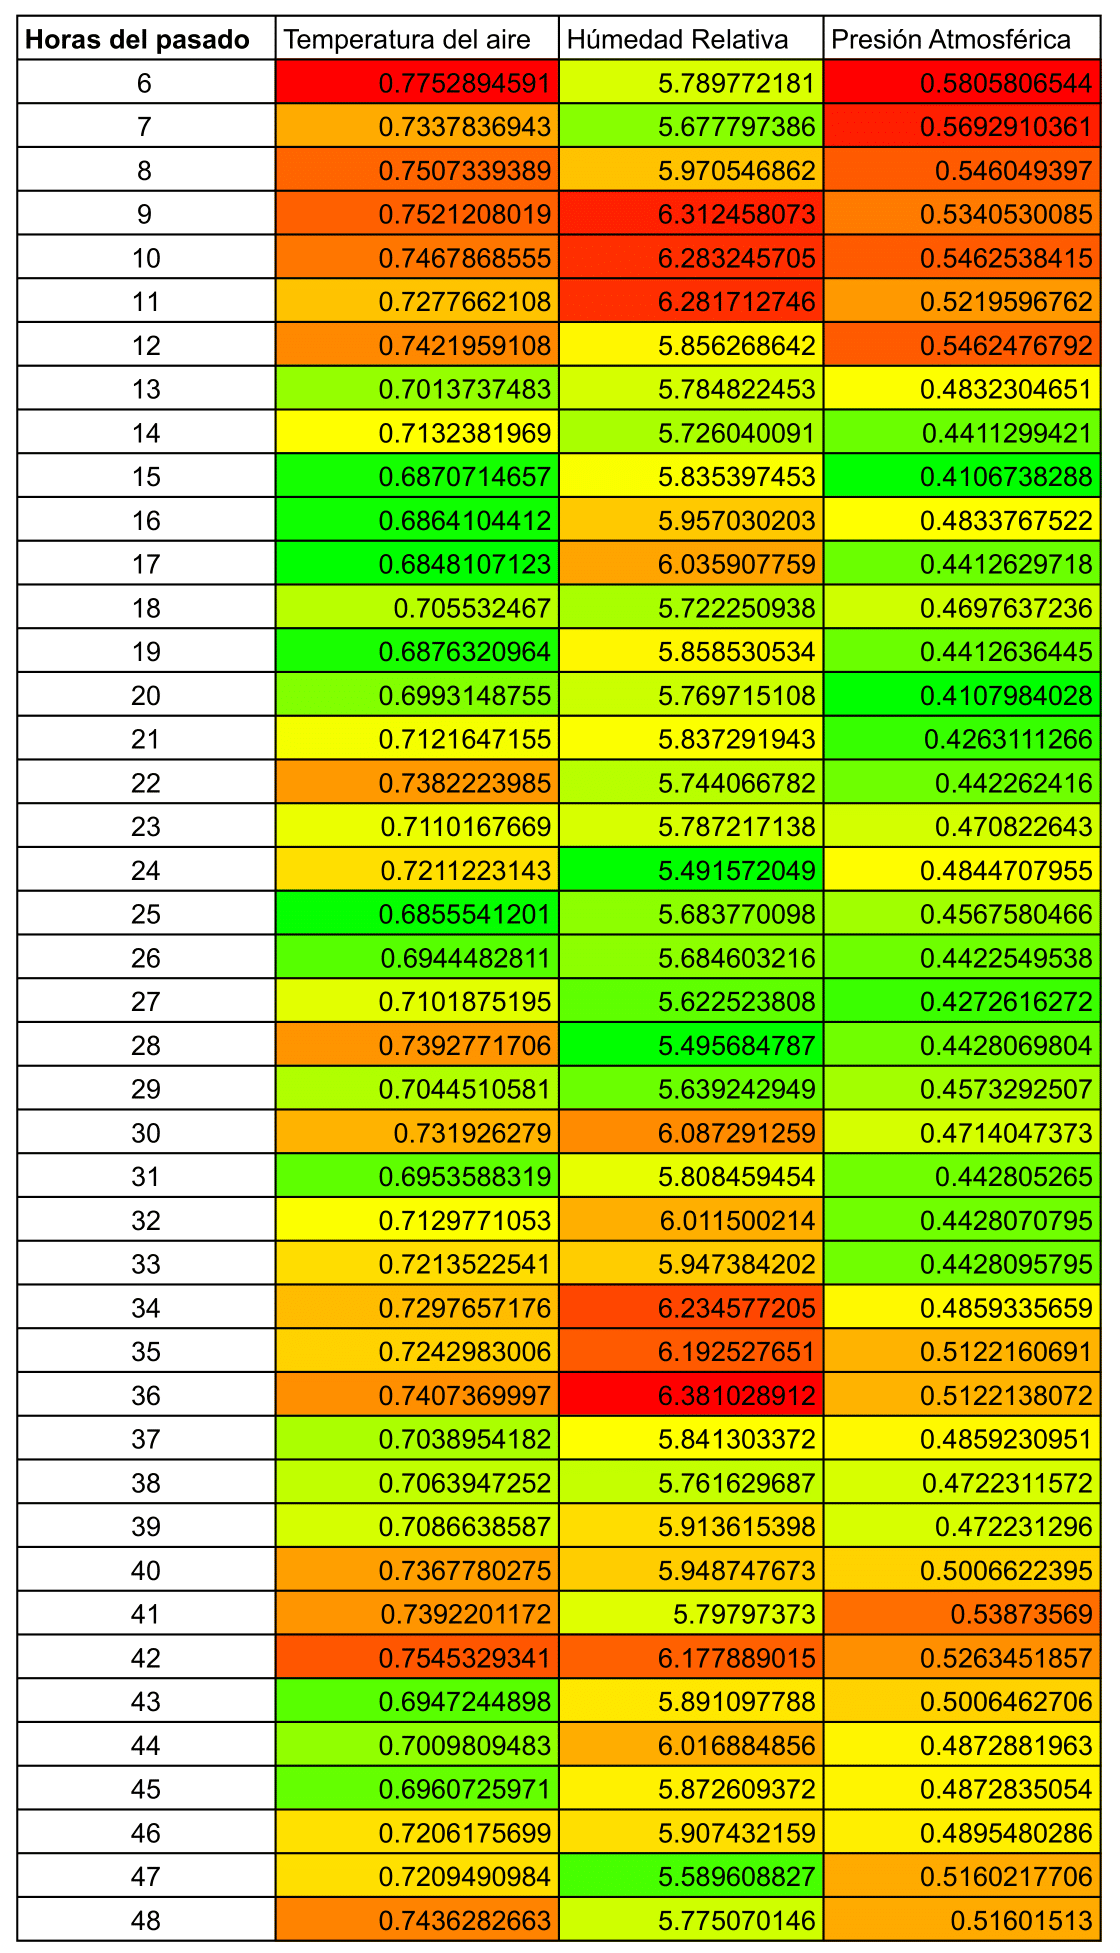
\includegraphics[width=0.7\textwidth]{images/past_window_size.png}
    \caption{Resultados del estudio del error RMSE del modelo LSTM en función del tamaño de la ventana }
    \label{window_size}
\end{figure}

Observando estos datos, se puede detectar un patrón en el que los modelos de 12 o menos horas dan peores resultados, 
mientras que el intervalo óptimo parece estar entre 15 y 26 horas, descendiendo los resultados a partir de las 30 horas.


\subsection{Uso de ruido}
Se plantea la hipótesis de que añadir un cierto ruido a los datos a medida que son consumidos en el entrenamiento puede favorecer la precisión del modelo al evitar el sobreajuste.
Esto es, se desea que el modelo en cada época no vea la misma muestra, sino que vea una versión ligeramente distinta. 

Para ello, se emplea el método .map del dataset de TensorFlow, que permite mapear otra función para su ejecución perezosa.
Se utiliza la función descrita en \ref{add_noise} sobre el conjunto de entrenamiento. En dicha función se aplica el ruido mediante una máscara
a los datos pasados de la variable y las covariables, sin alterar la codificación temporal. Además, se aplica ruido al valor objetivo $y$.

\begin{figure}[H]
{\small
\hrule
{\bf\small Pseudocódigo para agregar ruido}
\hrule
\begin{center}
\begin{tabbing}
\ 1: {\bf Función}\={\bf add\_noise}($x$, $y$, $covariates\_indexes$): \\
\ 2: \> Desempaquetar $x$ en \= $past,\, fut$ \\
\ 3: \> \# Generar ruido sobre las covariables \\
\ 4: \> $cov\_noise$ = noise\_distribution($past$, NOISE\_STD) \\
\ 5: \> \# Construir máscara de características afectadas \\
\ 6: \> $n\_features$ = shape($past$)[-1] \\
\ 7: \> $mask$ = ceros($(n\_features)$) \\
\ 8: \> $mask$[ $covariates\_indexes$ ] = 1 \\
10: \> $mask$ = reshape($mask$, $(1,1,n\_feat)$)  \# redimensión para aplicar al lote \\
11: \> \# Aplicar ruido sólo en características seleccionadas \\
12: \> $past\_noise$ = $cov\_noise \times mask$ \\
13: \> \# Generar ruido sobre la variable objetivo. \\
14: \> $target\_noise$ = noise\_distribution($y$, NOISE\_STD) \\
15: \> \# Retornar tupla con datos ruidosos y futuro sin modificar \\
16: \> {\bf Retornar}\ ( $(past + past\_noise),\, fut$ ),\ $y + target\_noise$ \\
\end{tabbing}
\end{center}
}
\hrule
\caption{Pseudocódigo de la función \texttt{add\_noise}}
\label{add_noise}
\end{figure}


Se prueban distintos valores de ruido y varias distribuciones: normal y una triangular, con menor desviación, construida mediante dos distribuciones uniformes.
Ejemplos de los datos con el ruido aplicado se pueden ver en las figuras \ref{noise1} y \ref{noise2}, donde se muestran los valores originales en continua, y los 
modificados con ruido en discontinua. También se experimenta aplicando coeficientes de ruido distintos a las covariables 
y a la variable objetivo. Se observa que un ruido menor al de las covariables en la variable objetivo mejora los resultados frente a usar el mismo valor.

\begin{figure}[H]
    \centering
    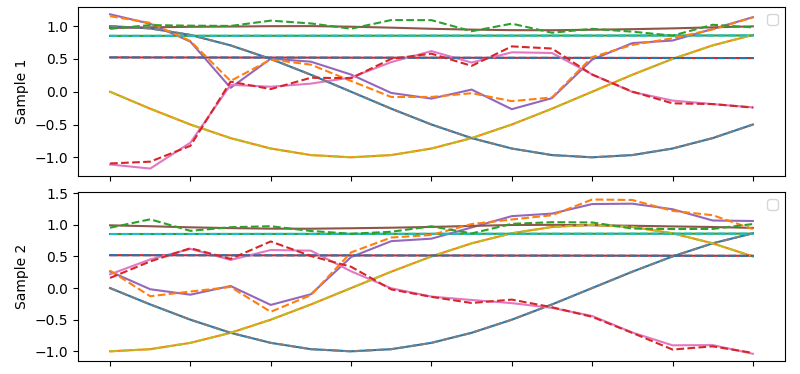
\includegraphics[width=0.7\textwidth]{images/noise_past_data.png}
    \caption{Datos pasados de 2 muestras con ruido.}
    \label{noise1}
\end{figure}

\begin{figure}[H]
    \centering
    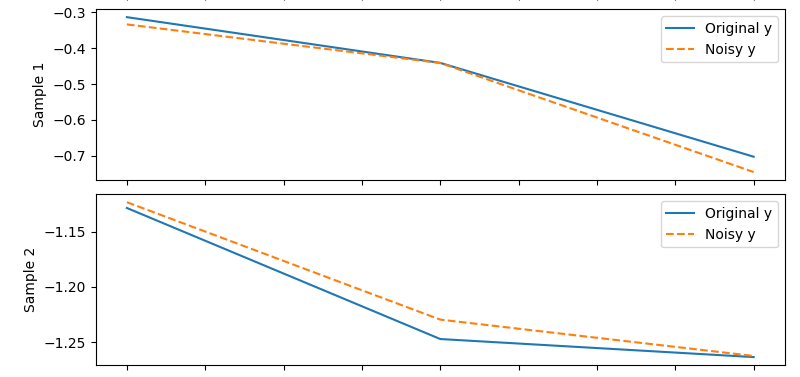
\includegraphics[width=0.7\textwidth]{images/noise_y.png}
    \caption{Valores objetivo de 2 muestras con ruido.}
    \label{noise2}
\end{figure}

Sin embargo, en la práctica se constata que el ruido no mejora los resultados de los modelos. Esto puede deberse a que las series exhiben una tendencia muy fuerte, 
que la inclusión del ruido no es capaz de modificar, puesto que sería necesario un ruido tan elevado que se perdería el valor de los datos.

\section{Modelos y Resultados}
\label{sec:resultados}
Cada variable tiene sus propias características y patrones, por lo que se desarrollan modelos LSTM específicos para cada una de ellas. 
Además, en el caso de la temperatura del aire, se estudia con mayor profundidad y se desarrollan modelos específicos para cada horizonte de predicción.
Los resultados obtenidos corresponden al mejor modelo de 10 entrenamientos. Se muestra el error RMSE de la validación cruzada, así como sobre los conjuntos de test.

\subsection{Temperatura del aire}
Los modelos, ajustados para cada horizonte de predicción, se muestran en los pseudocódigos \ref{lstm_model_temp_3h}, \ref{lstm_model_temp_6h}, \ref{lstm_model_temp_12h}.
Los resultados obtenidos se muestran en la tabla \ref{temp_results}. Observamos que los datos de test son similares a los de validación, 
lo que indica que el modelo generaliza bien.

\begin{figure}[H]
{\small
\hrule
{\bf\small Pseudocódigo para el modelo de temperatura a 3 horas}
\hrule
\begin{center}
\begin{tabbing}
\ 1: {\bf Fun}\={\bf ción construir\_modelo}($past\_shape$, $future\_shape$, $forecast_length$, $learning\_rate$): \\
\ 2: \> \# Definir capas de entrada \\
\ 3: \> $entrada\_pasado$ = Input(shape=$past\_shape$) \\
\ 4: \> $entrada\_futuro$ = Input(shape=$future\_shape$) \\
\ 5: \> \# Procesar datos pasados con BiLSTM \\
\ 6: \> $past\_lstm$ = BiLSTM(unidades=65, return\_sequences=False)($entrada\_pasado$) \\
\ 7: \> \# Procesar datos futuros con LSTM \\
\ 8: \> $future\_lstm$ = LSTM(unidades=4, return\_sequences=False)($entrada\_futuro$) \\
\ 9: \> \# Aplanar la entrada futura como residuo \\
10: \> $residuo\_futuro$ = Flatten()($entrada\_futuro$) \\
11: \> \# Combinar todas las salidas \\
12: \> $merged$ = concatenar($past\_lstm$, $future\_lstm$, $residuo\_futuro$) \\
13: \> $salida$ = Dense(unidades=$forecast_length$)($merged$) \\
14: \> \# Construir y compilar el modelo \\
15: \> modelo = Modelo(entradas=[ $entrada\_pasado$, $entrada\_futuro$ ], salidas=$salida$) \\
16: \> compilar(modelo, optimizador=Adam($learning\_rate$), pérdida='MSE') \\
27: \> {\bf Retornar} modelo \\
\end{tabbing}
\end{center}
}
\hrule
\caption{Pseudocódigo para el modelo de temperatura a 3 horas}
\label{lstm_model_temp_3h}
\end{figure}

\begin{figure}[H]
{\small
\hrule
{\bf\small Pseudocódigo para el modelo de temperatura a 6 horas}
\hrule
\begin{center}
\begin{tabbing}
\ 1: {\bf Fun}\={\bf ción construir\_modelo}($past\_shape$, $future\_shape$, $forecast\_length$, $learning\_rate$): \\
\ 2: \> \# Definir capas de entrada \\
\ 3: \> $entrada\_pasado$ = Input(shape=$past\_shape$) \\
\ 4: \> $entrada\_futuro$ = Input(shape=$future\_shape$) \\
\ 5: \> \# Procesar datos pasados con BiLSTM y proyección densa \\
\ 6: \> $past\_lstm$ = BiLSTM(unidades=65, return\_sequences=False)($entrada\_pasado$) \\
\ 7: \> $past\_lstm$ = Dense(unidades=65)($past\_lstm$) \\
\ 8: \> \# Procesar datos futuros con LSTM \\
\ 9: \> $decoder\_lstm$ = LSTM(unidades=4, return\_sequences=False)($entrada\_futuro$) \\
10: \> \# Aplanar la entrada futura como residuo \\
11: \> $residuo\_futuro$ = Flatten()($entrada\_futuro$) \\
12: \> \# Combinar todas las salidas \\
13: \> $merged$ = concatenar($past\_lstm$, $decoder\_lstm$, $residuo\_futuro$) \\
14: \> \# Capas densas finales \\
15: \> $merged$ = Dense(unidades=$4 \times forecast\_length$)($merged$) \\
16: \> $salida$ = Dense(unidades=$forecast\_length$)($merged$) \\
\end{tabbing}
\end{center}
}
\hrule
\caption{Pseudocódigo para el modelo de temperatura a 6 horas}
\label{lstm_model_temp_6h}
\end{figure}

\begin{figure}[H]
{\small
\hrule
{\bf\small Pseudocódigo para el modelo de temperatura a 12 horas}
\hrule
\begin{center}
\begin{tabbing}
\ 1: {\bf Fun}\={\bf ción construir\_modelo}($past\_shape$, $future\_shape$, $forecast\_length$, $learning\_rate$): \\
\ 2: \> \# Definir capas de entrada \\
\ 3: \> $entrada\_pasado$ = Input(shape=$past\_shape$) \\
\ 4: \> $entrada\_futuro$ = Input(shape=$future\_shape$) \\
\ 5: \> \# Procesar datos pasados con BiLSTM y proyección densa \\
\ 6: \> $past\_lstm$ = BiLSTM(unidades=65, return\_sequences=False)($entrada\_pasado$) \\
\ 7: \> $past\_lstm$ = Dense(unidades=65)($past\_lstm$) \\
\ 8: \> \# Procesar datos futuros con LSTM \\
\ 9: \> $future\_lstm$ = LSTM(unidades=4, return\_sequences=False)($entrada\_futuro$) \\
10: \> \# Aplanar la entrada futura como residuo \\
11: \> $residuo\_futuro$ = Flatten()($entrada\_futuro$) \\
12: \> \# Combinar todas las salidas \\
13: \> $merged$ = concatenar($past\_lstm$, $future\_lstm$ , $residuo\_futuro$) \\
14: \> \# Capa densa de salida \\
15: \> $salida$ = Dense(unidades=$forecast\_length$)($merged$) \\
\end{tabbing}
\end{center}
}
\hrule
\caption{Pseudocódigo para el modelo de temperatura a 12 horas}
\label{lstm_model_temp_12h}
\end{figure}


\begin{table}[h!]
\centering
\begin{tabular}{|l|c|c|c|}
\hline
\multicolumn{1}{|c|}{} & \multicolumn{3}{c|}{\textbf{Horizonte de predicción (horas)}} \\
\hline
\textbf{Datos} & \textbf{3} & \textbf{6} & \textbf{12} \\
\hline
Validación   &      0.6792           &     0.8543       &         1.0632            \\
\hline
Garachico    &        0.8234         &      1.0677            &         1.3423            \\
\hline
Santa Cruz &       0.6711          &    0.7892          &          0.9244           \\
\hline
\end{tabular}
\caption{Resultados del modelo LSTM para la temperatura del aire}
\label{temp_results}
\end{table}


\subsection{Humedad relativa}

Se emplea el modelo descrito en la figura \ref{lstm_model_hum}, que consiste en una LSTM bidireccional seguida de una capa densa para los datos pasados, una
capa densa para los datos futuros y dos capa densas apiladas para la salida.

\begin{figure}[H]
{\small
\hrule
{\bf\small Pseudocódigo del modelo BiLSTM para la humedad relativa}
\hrule
\begin{center}
\begin{tabbing}
\ 1: {\bf Fun}\={\bf ción construir\_modelo}($past\_shape$, $future\_shape$, $forecast\_length$, $learning\_rate$): \\
\ 2: \> \# Definir capas de entrada \\
\ 3: \> $entrada\_pasado$ = Input(shape=$past\_shape$) \\
\ 4: \> $entrada\_futuro$ = Input(shape=$future\_shape$) \\
\ 5: \> \# Codificador del pasado con BiLSTM y proyección \\
\ 6: \> $past\_lstm$ = BiLSTM(unidades=42, return\_sequences=False)($entrada\_pasado$) \\
\ 7: \> $past\_lstm$ = Dense(unidades=20)($past\_lstm$) \\
\ 8: \> \# Variables futuras: aplanar y proyectar \\
\ 9: \> $future\_dense$ = Flatten()($entrada\_futuro$) \\
10: \> $future\_dense$ = Dense(unidades=4)($future\_dense$) \\
11: \> \# Residuo adicional de variables exógenas \\
12: \> $residuo\_futuro$ = Flatten()($entrada\_futuro$) \\
13: \> \# Combinar todas las salidas \\
14: \> $merged$ = concatenar($past\_lstm$, $future\_dense$, $residuo\_futuro$) \\
15: \> \# Capas densas finales para predicción \\
16: \> $merged$ = Dense(unidades=6 $\times$ $forecast\_length$)($merged$) \\
17: \> $salida$ = Dense(unidades=$forecast\_length$)($merged$) \\
\end{tabbing}
\end{center}
}
\hrule
\caption{Pseudocódigo del modelo BiLSTM para la humedad relativa}
\label{lstm_model_hum}
\end{figure}


\begin{table}[h!]
\centering
\begin{tabular}{|l|c|c|c|}
\hline
\multicolumn{1}{|c|}{} & \multicolumn{3}{c|}{\textbf{Horizonte de predicción (horas)}} \\
\hline
\textbf{Datos} & \textbf{3} & \textbf{6} & \textbf{12} \\
\hline
Validación   &     5.7526            &    7.0293            &    8.5234                 \\
\hline
Garachico    &     5.7889            &     7.7114           &    9.1482                 \\
\hline
Santa Cruz &       4.6226          &   5.0627               &    6.0066                 \\
\hline
\end{tabular}
\caption{Resultados del modelo LSTM para la humedad relativa}
\label{hum_results}
\end{table}


\subsection{Presión atmosférica}
Se emplea el modelo descrito en la figura \ref{lstm_model_pres}, similar al empleado para la humedad relativa.
\begin{figure}[H]
{\small
\hrule
{\bf\small Pseudocódigo del modelo BiLSTM para la presión atmosférica}
\hrule
\begin{center}
\begin{tabbing}
\ 1: {\bf Fun}\={\bf ción construir\_modelo}($past\_shape$, $future\_shape$, $forecast\_length$, $learning\_rate$): \\
\ 2: \> \# Definir capas de entrada \\
\ 3: \> $entrada\_pasado$ = Input(shape=$past\_shape$) \\
\ 4: \> $entrada\_futuro$ = Input(shape=$future\_shape$) \\
\ 5: \> \# Codificador pasado con BiLSTM + capa densa \\
\ 6: \> $past\_lstm$ = BiLSTM(unidades=56, return\_sequences=False)($entrada\_pasado$) \\
\ 7: \> $past\_lstm$ = Dense(unidades=58)($past\_lstm$) \\
\ 8: \> \# Variables futuras: aplanar y proyectar con Dense \\
\ 9: \> $future\_dense$ = Flatten()($entrada\_futuro$) \\
10: \> $future\_dense$ = Dense(unidades=4)($future\_dense$) \\
11: \> \# Aplanar también como residuo \\
12: \> $residuo\_futuro$ = Flatten()($entrada\_futuro$) \\
13: \> \# Combinar todas las salidas \\
14: \> $merged$ = concatenar($past\_lstm$, $future\_dense$, $residuo\_futuro$) \\
15: \> \# Capa densa intermedia y salida final \\
16: \> $merged$ = Dense(unidades=6 $\times$ $forecast\_length$)($merged$) \\
17: \> $salida$ = Dense(unidades=$forecast\_length$)($merged$) \\
\end{tabbing}
\end{center}
}
\hrule
\caption{Pseudocódigo del modelo BiLSTM para la presión atmosférica}
\label{lstm_model_pres}
\end{figure}


\begin{table}[h!]
\centering
\begin{tabular}{|l|c|c|c|}
\hline
\multicolumn{1}{|c|}{} & \multicolumn{3}{c|}{\textbf{Horizonte de predicción (horas)}} \\
\hline
\textbf{Datos} & \textbf{3} & \textbf{6} & \textbf{12} \\
\hline
Validación   &   0.3908           &    0.5541        &   0.7963          \\
\hline
Garachico    & 0.6783             &     0.8761       &     1.2887               \\
\hline
Santa Cruz &    0.4077            &     0.6341       &    0.9809                 \\
\hline
\end{tabular}
\caption{Resultados del modelo LSTM para la presión atmosférica}
\label{pres_results}
\end{table}


\subsection{Evaluación de los resultados}
Se decide graficar las predicciones para tener una mejor comprensión de los resultados obtenidos. Se muestran comparativas entre las predicciones a 12 horas y los valores
reales para el conjunto de test de Santa Cruz de Tenerife. En las figuras \ref{temp_sct}, \ref{pres_sct} se ven ejemplos de predicciones muy acertadas. 
En el caso de la figura \ref{hum_sct}, se observa que el modelo predice adecuadamente la tendencia, si bien existe un valle repentino, que quizás pudiera ser ruido del sensor.
Por otra parte, existen situaciones en las que los resultados se alejan de los valores reales, como se observa en la figura \ref{temp_sct_error}. Esto puede deberse
a la naturaleza de las variables, con comportamientos difíciles de predecir en ocasiones, o por otra parte, a la falta de contexto e información necesaria para hacer una predicción precisa.

\begin{figure}
    \centering
    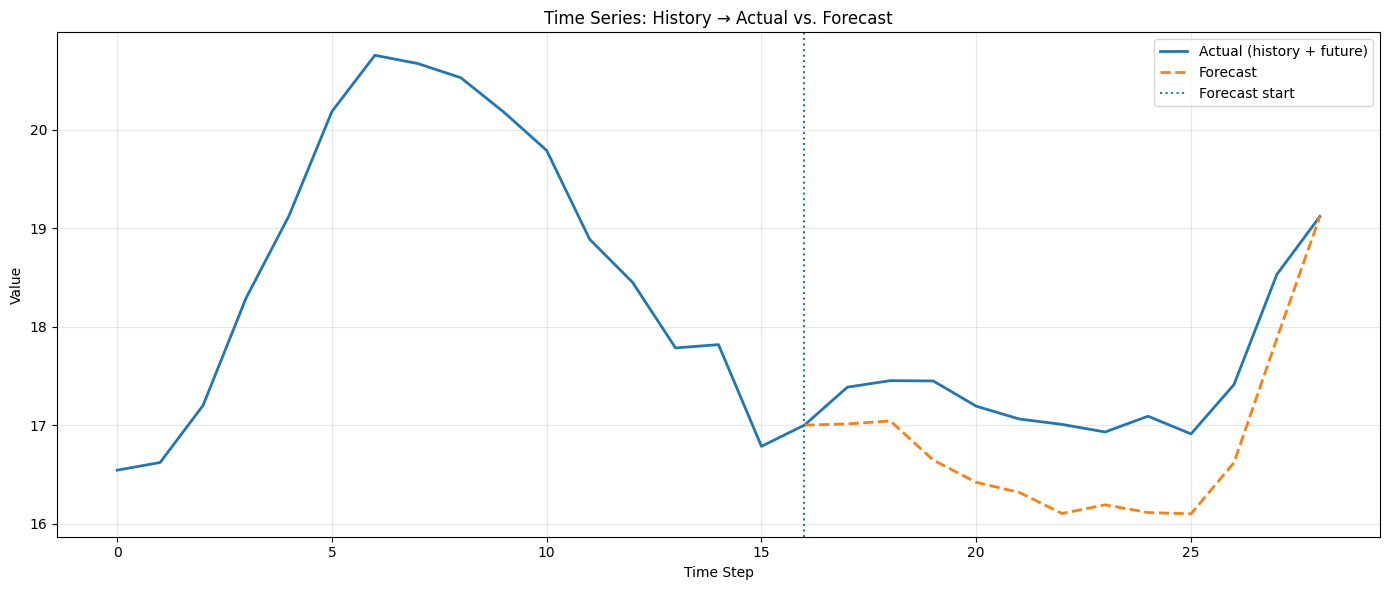
\includegraphics[width=0.7\textwidth]{images/grafico_f12_temp.png}
    \caption{Predicciones de temperatura del aire en Santa Cruz de Tenerife}
    \label{temp_sct}
\end{figure}

\begin{figure}
    \centering
    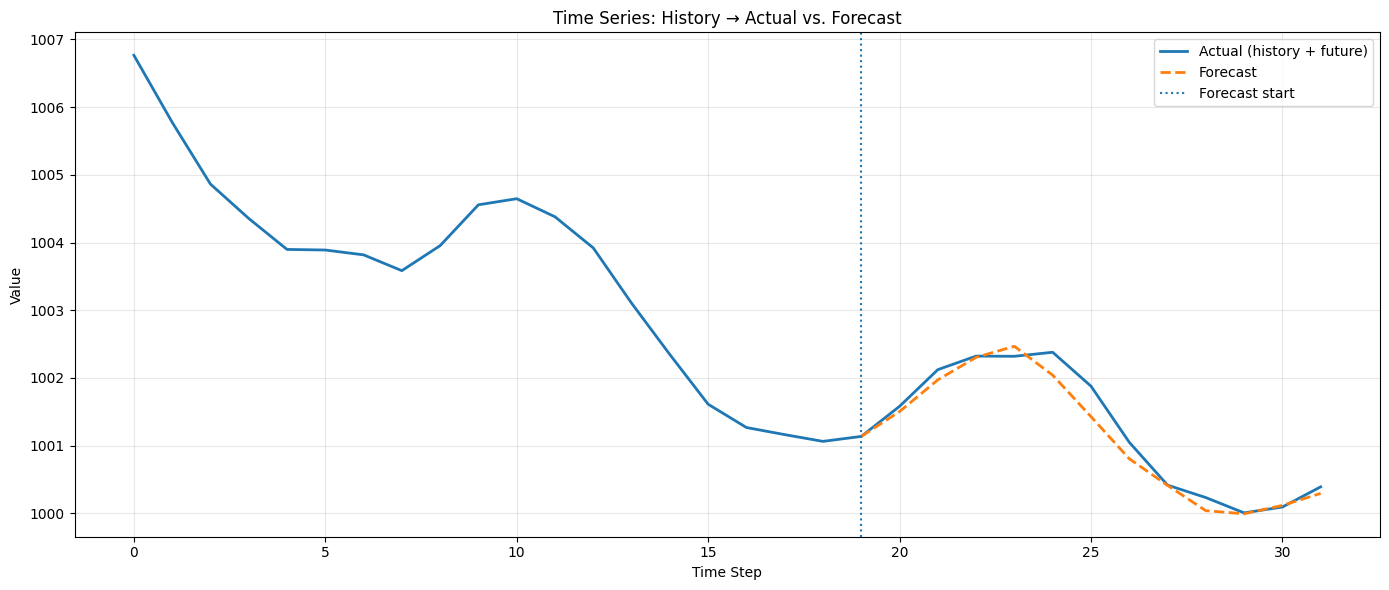
\includegraphics[width=0.7\textwidth]{images/grafico_f12_pres.png}
    \caption{Predicciones de presión atmosférica en Santa Cruz de Tenerife}
    \label{pres_sct}
\end{figure}    

\begin{figure}
    \centering
    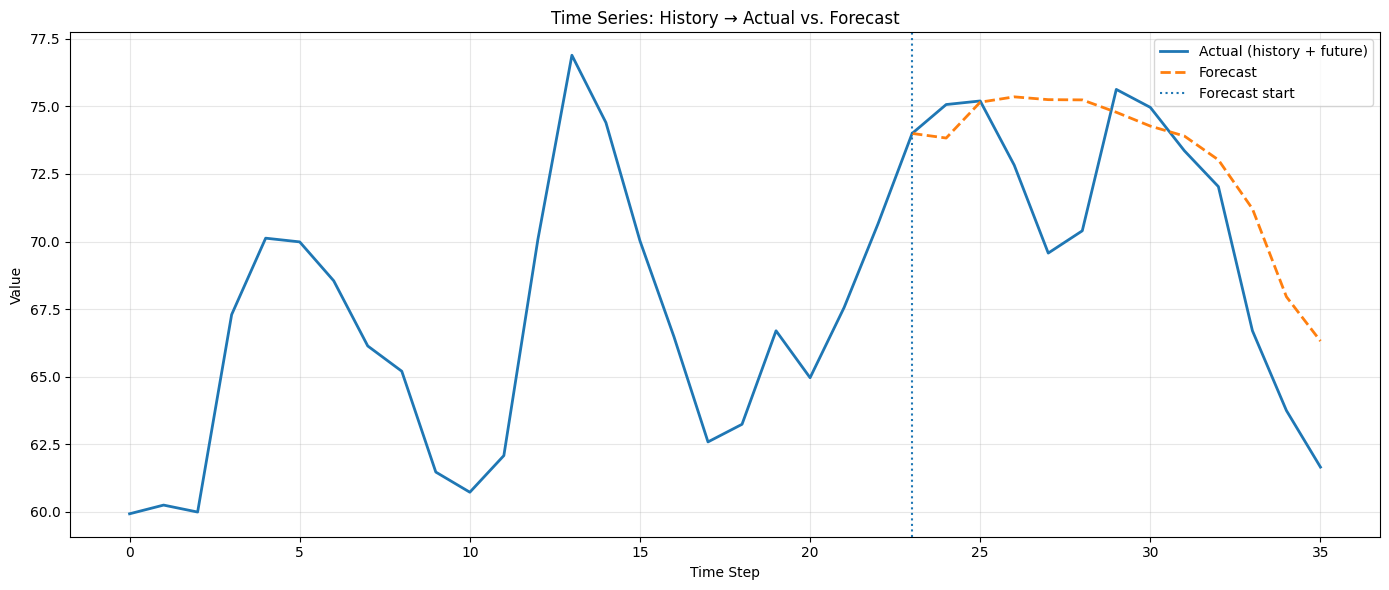
\includegraphics[width=0.7\textwidth]{images/grafico_f12_hum.png}
    \caption{Predicciones de humedad relativa en Santa Cruz de Tenerife}
    \label{hum_sct}
\end{figure}

\begin{figure}
    \centering
    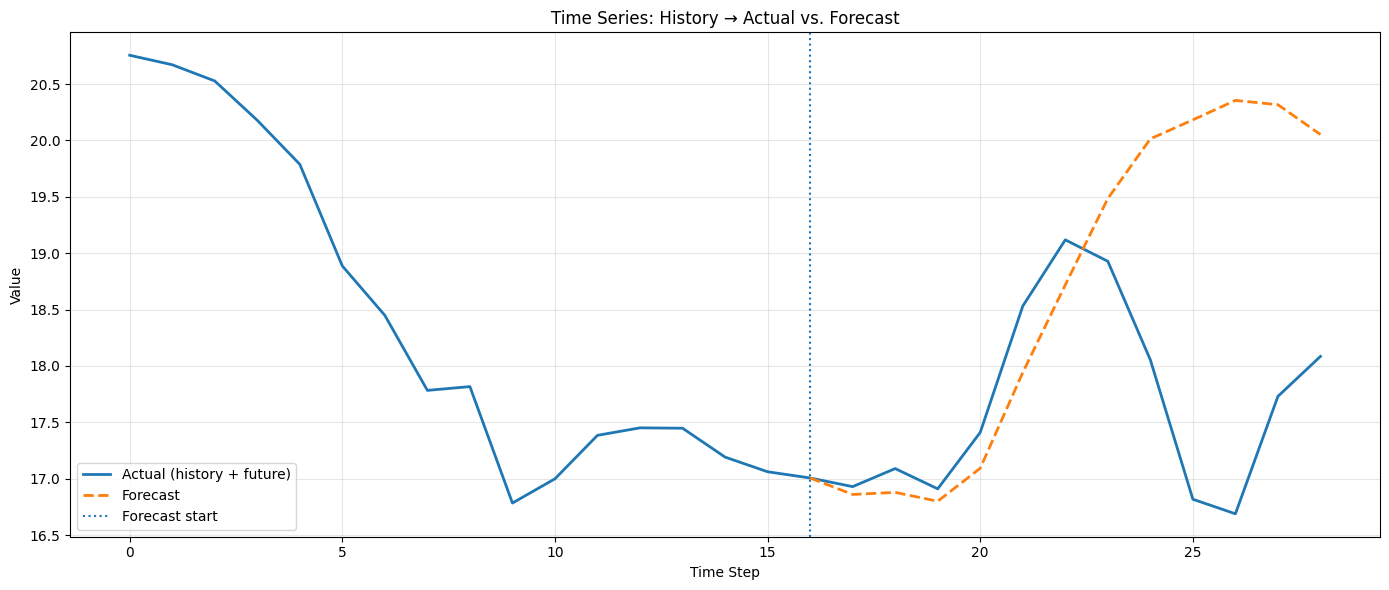
\includegraphics[width=0.7\textwidth]{images/grafico_f12_temp_mal.png}
    \caption{Predicciones de temperatura del aire en Santa Cruz de Tenerife 2}
    \label{temp_sct_error}
\end{figure}

En general, los resultados son satisfactorios, destacando la capacidad de los modelos para predecir adecuadamente las tendencias de las variables.

Para contextualizar los resultados obtenidos, se comparan con otros trabajos similares.
Esta comparativa es meramente orientativa, debido a que las condiciones meteorológicas pueden variar entre distintas ubicaciones.

Se toman como referencia los resultados del estudio de Haque et al. \cite{haque2021}, que emplea modelos de aprendizaje profundo para la predicción de la temperatura 
en las próximas 6 horas en la ciudad de Pekín. Además, se evalúa el mismo modelo en otras ciudades, como Toronto o Las Vegas. 

En dicho estudio, el mejor RMSE para 6 horas obtenido era de 1.691, mientras que con nuestro modelo se obtiene un RMSE de 0.8543, lo que sugiere que el modelo es capaz de predecir la temperatura del aire con una precisión considerablemente mayor. 
Además, en el estudio citado, para las ciudades no usadas en el entrenamiento, el RMSE se sitúa entre 1.4 y 2.7, siendo en nuestro caso de 1.0677 y 0.7892 para las estaciones consideradas,
lo que valida la capacidad de nuestro modelo para generalizar a otras ubicaciones.


%%%%%%%%%%%%%%%%%%%%%%%%%%%%%%%%%%%%%%%%%%%%%%%%%%%%%%%%%
\newpage{\pagestyle{empty}}
\thispagestyle{empty}

\chapter{\LARGE Despliegue}
\label{chapter:cuatro}


Se desea realizar un despliegue del proyecto, de forma que los modelos de predicción sean accesibles mediante una interfaz web. Específicamente, se plantea que cualquier usuario 
pueda seleccionar una de las estaciones de GRAFCAN, y a partir de la misma, que la aplicación web devuelva la predicción de alguna de las variables meteorológicas en las próximas horas. 
Se decide arbitrariamente acotar la predicción a la variable de temperatura y a las próximas 6 horas.

Se realiza una interfaz web sencilla como front-end, y un back-end que maneje la carga de trabajo de predicción. Las predicciones se ejecutan de forma asíncrona 
para no bloquear la experiencia del usuario y permitir un cierto nivel de paralelismo.

\section{Front-end}
Tras valorar distintas opciones, se decide emplear React como framework para el front-end. Se elige por su facilidad de uso y la gran cantidad de librerías que existen para este.
Se emplea Typescript para la codificación, al ser una alternativa más robusta a Javascript, y que permite detectar errores de forma más sencilla.

Se crea una aplicación de una sola página (Single Page Application) que permite al usuario buscar y seleccionar una estación de GRAFCAN. Una vez seleccionada,
se envía una petición al back-end para obtener la predicción.

Las características de la aplicación son las siguientes:
\begin{itemize}
    \item \textbf{Selector de estaciones}: Permite al usuario seleccionar una estación de GRAFCAN. Se agrupan las estaciones por ubicación para facilitar la búsqueda.
    \item \textbf{Visualización de sensores}: Una vez seleccionada la estación, se muestran los sensores disponibles en la misma. 
    \item \textbf{Indicadores visuales de estado de la predicción}: Se utilizan indicadores visuales para mostrar el estado de la predicción. Estos indicadores permiten al usuario saber si la predicción está en curso, ha fallado o se ha completado con éxito.
\end{itemize}


Para el desarrollo de la aplicación es necesario crear una serie de elementos denominados \char`\"componentes". Estos componentes son bloques de código que 
permiten crear una interfaz de usuario modular y reutilizable. En este caso, se crean, entre otros:
\begin{itemize}
    \item \textbf{Dashboard}: Componente principal de la aplicación. Se encarga de gestionar el estado de la aplicación y de renderizar los demás componentes.
    \item \textbf{Selector de estaciones}: permite al usuario seleccionar una estación de GRAFCAN, ordenadas por ubicación geográfica.
    \item \textbf{Gráficas de sensor}: Se utilizan para mostrar los datos históricos de la estación seleccionada. 
    \item \textbf{Estado de predicción}: Indicadores permiten al usuario saber si la predicción está en curso, ha fallado o se ha completado con éxito.
    \item \textbf{Información de estación}: Muestra información detallada de la estación seleccionada, incluyendo los sensores disponibles y su estado.
\end{itemize}

La figura \ref{frontend_loading} muestra un ejemplo de la interfaz web mientras se recuperan los datos de una estación, la figura 
\ref{frontend_loaded} contiene el resultado y en \ref{frontend_prediction} se muestra el resultado de una predicción.

\begin{figure}[H]
    \centering
    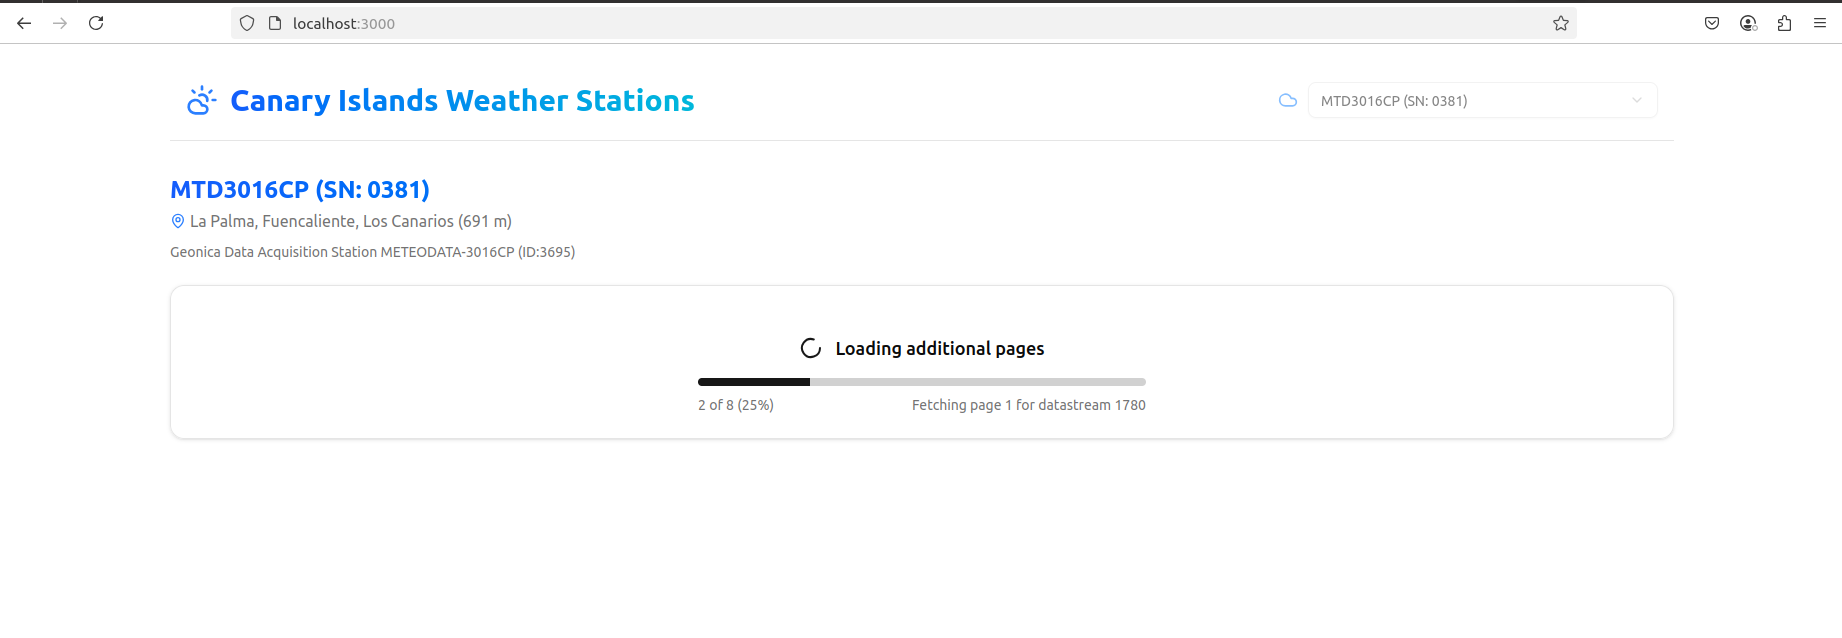
\includegraphics[width=0.9\textwidth]{images/frontend_loading.png}
    \caption{Interfaz web. Carga de datos de una estación}
    \label{frontend_loading}
\end{figure}

\begin{figure}[H]
    \centering
    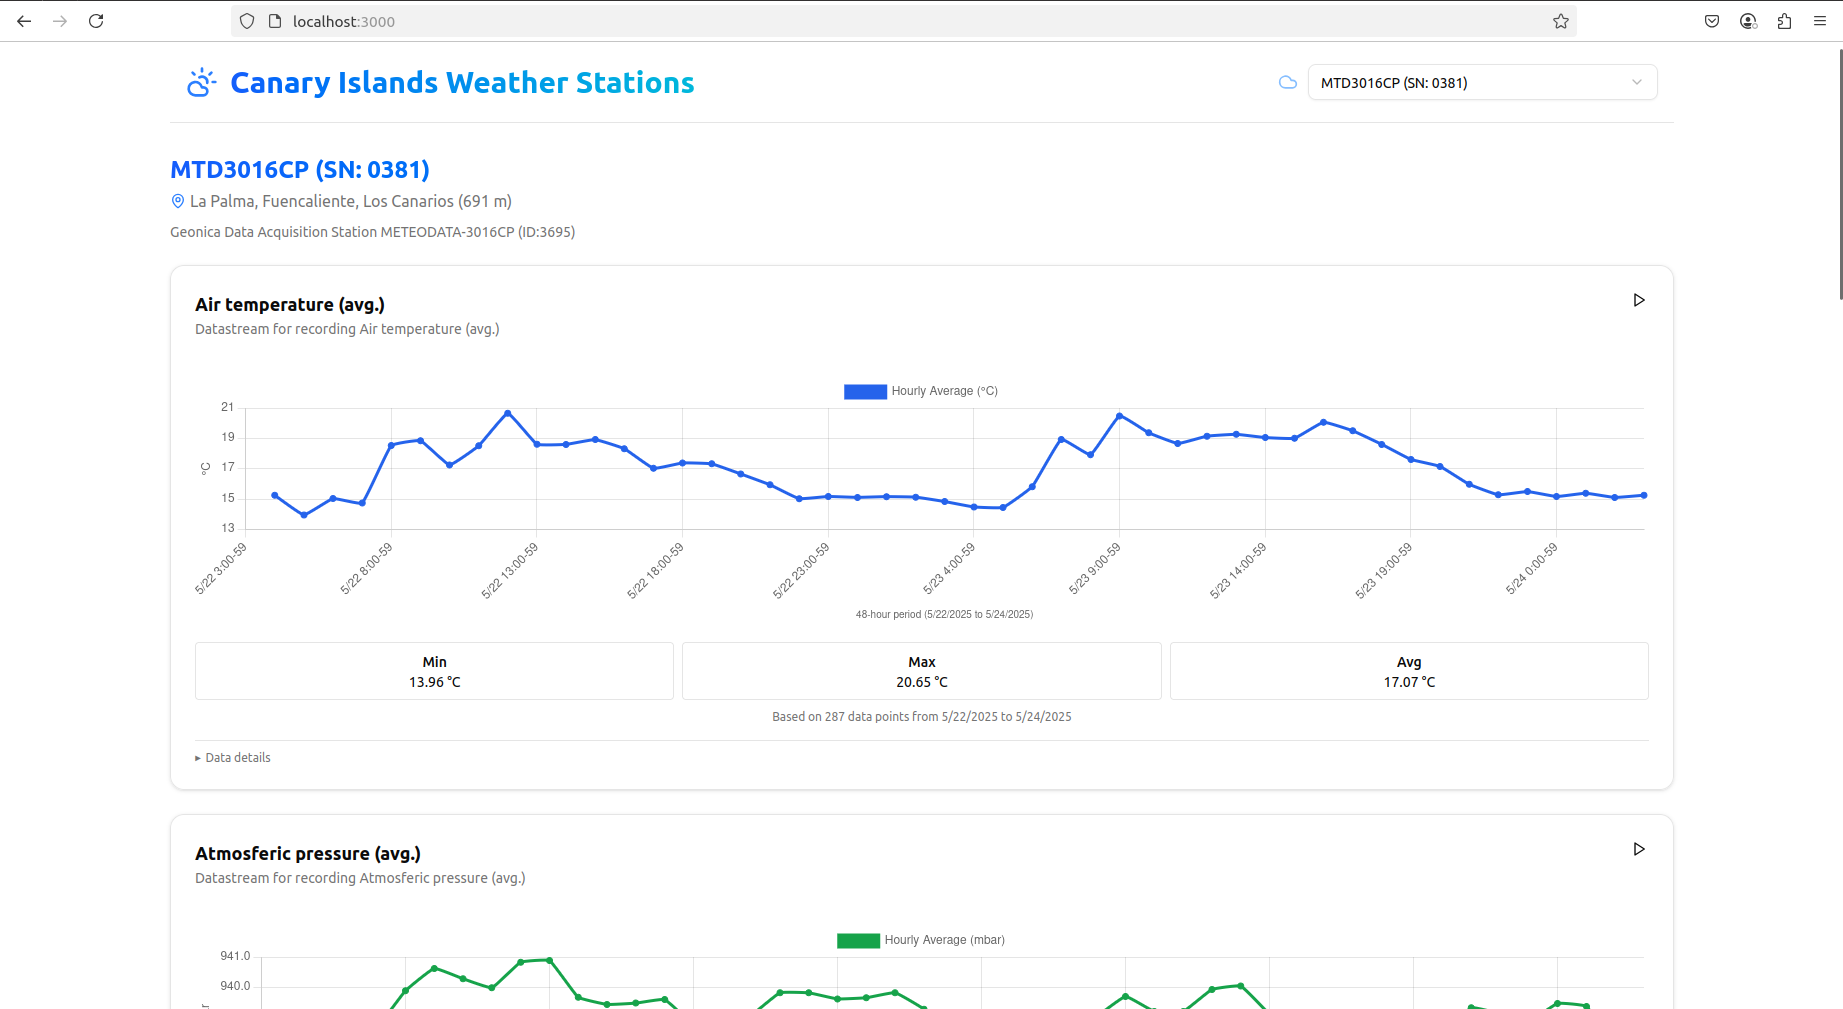
\includegraphics[width=0.9\textwidth]{images/frontend_loaded.png}
    \caption{Interfaz web. Gráfica con datos de una estación}
    \label{frontend_loaded}
\end{figure}

\begin{figure}[H]
    \centering
    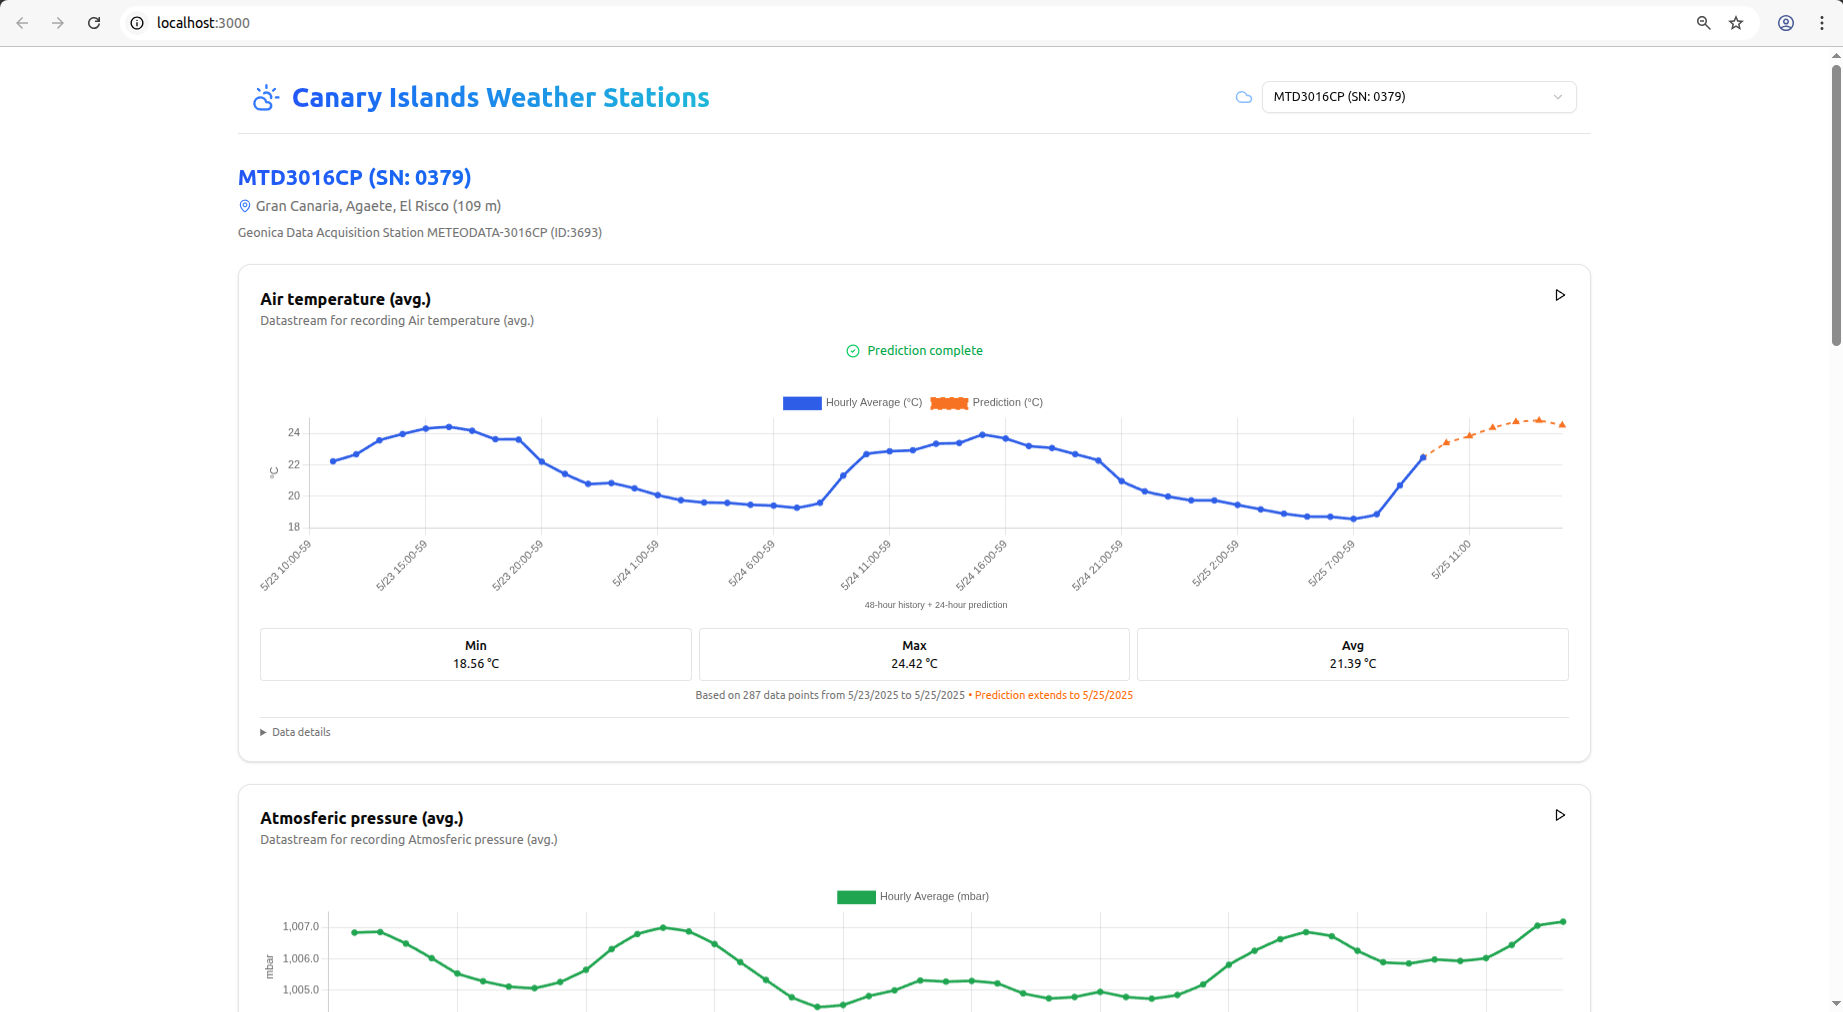
\includegraphics[width=0.9\textwidth]{images/frontend_prediction_6.png}
    \caption{Interfaz web. Resultado de una predicción}
    \label{frontend_prediction}
\end{figure}


\section{Back-end}

\begin{itemize}
    \item \textbf{FastAPI}: Se trata de un framework web para construir APIs en Python, que facilita crear servicios RESTful con alto rendimiento. Se emplea para gestionar las peticiones de predicción.
    \item \textbf{Worker Celery}: Como nodo trabajador se emplea Celery, una biblioteca de Python para ejecutar tareas asíncronas y distribuir trabajos en segundo plano, ideal para procesar tareas largas o programadas sin bloquear la aplicación principal. 
    Se utiliza como sistema de tareas asíncronas para evitar bloquear el servidor web durante la ejecución de las predicciones. El worker carga el modelo LSTM previamente entrenado al iniciarse, utilizando los pesos almacenados localmente. 
    \item \textbf{Redis}: Se utiliza como broker de tareas para Celery. Permite almacenar y gestionar las tareas encoladas, facilitando la comunicación entre el servidor web y los workers.
\end{itemize}

Esta arquitectura, que se muestra en la figura \ref{deploy_scheme}, facilita el despliegue, escalabilidad y mantenimiento del sistema, permitiendo además la ejecución paralela de múltiples workers para atender una mayor carga de solicitudes.
\begin{figure}[H]
    \centering
    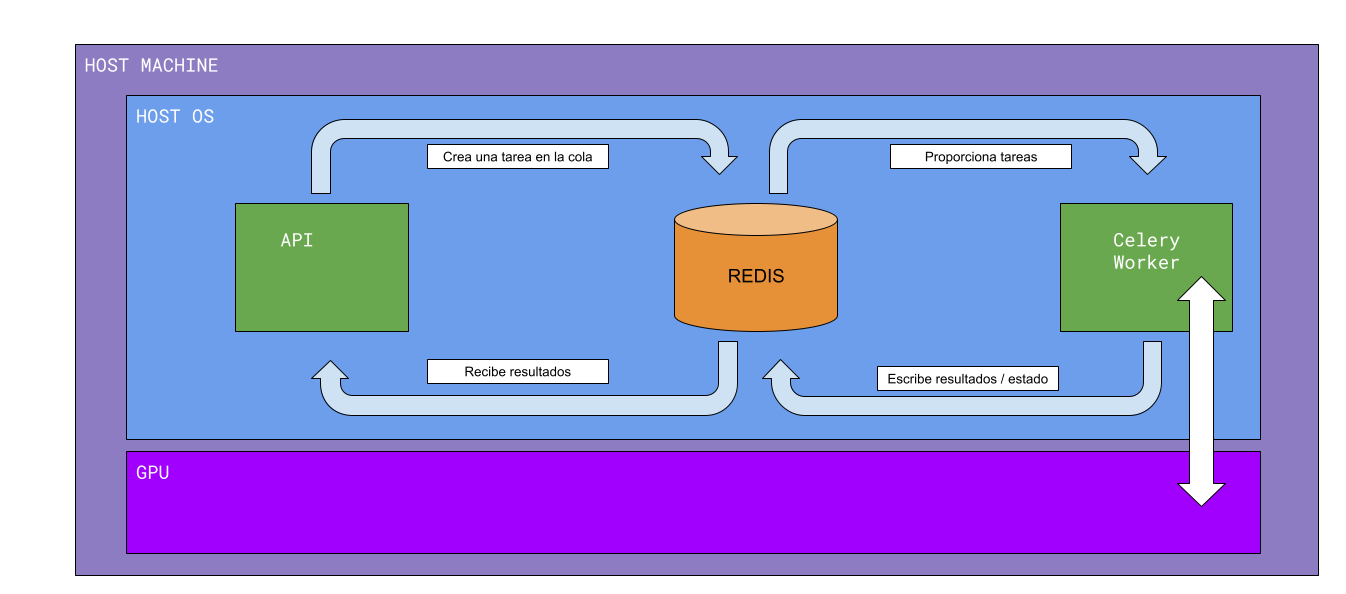
\includegraphics[width=0.9\textwidth]{images/esquema_despliegue.png}
    \caption{Esquema de la lógica del despliegue}
    \label{deploy_scheme}
\end{figure}

La API es responsable de validar y transformar los datos de entrada, preparar la estructura requerida por el modelo de predicción y coordinar la ejecución de las tareas de inferencia mediante Celery.

Los endpoints disponibles en la API son:

\begin{itemize}
    \item \textbf{POST $/$predict}:  recibe datos estructurados correspondientes a observaciones recientes de una estación. Estos datos se procesan para generar un tensor con forma [1, T, F], donde T representa el número de intervalos temporales considerados y F = 7 corresponde a las características de entrada (cuatro variables temporales codificadas mediante funciones seno y coseno para capturar patrones cíclicos diarios y anuales, y tres variables provenientes de sensores). A continuación, la solicitud es encolada como una tarea en Celery para su procesamiento.
    \item \textbf{GET $/$predict$/${job\_id}}: permite consultar el estado de la tarea asociada al identificador job\_id. En caso de que la predicción ya esté disponible, devuelve el resultado generado.
\end{itemize}
El procesamiento interno del back-end incluye la extracción de características temporales relevantes y la conversión de los datos a tensores NumPy que alimentan el modelo de predicción.


El flujo general de una petición de predicción es el siguiente:

\begin{itemize}
    \item El usuario selecciona una estación de GRAFCAN y un sensor específico en la interfaz web.
    \item El front-end recopila las observaciones de los últimos 48 intervalos horarios y envía esta información al back-end mediante el endpoint POST /predict.
    \item El back-end valida y transforma los datos, encolando la tarea en Celery.
    \item El worker procesa la tarea, ejecutando el modelo LSTM para obtener la predicción.
    \item El front-end consulta periódicamente el estado y resultado de la tarea mediante el endpoint GET /predict/{job\_id}.
    \item  Finalmente, el resultado se presenta visualmente, superponiéndose a las gráficas de las observaciones originales del sensor.
\end{itemize}



%%%%%%%%%%%%%%%%%%%%%%%%%%%%%%%%%%%%%%%%%%%%%%%%%%%%%%%%%
\newpage{\pagestyle{empty}}
\thispagestyle{empty}

\chapter{\LARGE Conclusiones y líneas futuras}
\label{chapter:Resultados}


En este trabajo se ha desarrollado un sistema de predicción de variables meteorológicas, capaz de generalizar y realizar predicciones de ubicaciones no vistas. 
Se han estudiado diversas alternativas en el ámbido del aprendizaje profundo, y se ha observado que los modelos LSTM son los que mejores resultados brindan de entre los modelos estudiados. Además,
se ha comprobado que estos resultados son buenos. Son mejores que los de modelos tradicionales para predicción de series temporales, y superan a los resultados de otras investigaciones 
recientes.

Se ha elaborado todo un flujo de trabajo, desde la obtención de datos, su tratamiento y limpieza, hasta la creación de los modelos de predicción. Y se han 
realizado extensas pruebas de distintas teorías y configuraciones, con el fin de obtener los mejores resultados para este problema.

Una de las consideraciones más llamativas, es que estudiando el tamaño de la ventana de datos pasados se observa que empleando pocas mediciones, máximoe un día, se obtienen mejores predicciones que
con períodos más extensos. Esto es particularmente útil puesto que permite reducir el número de mediciones necesarias para realizar una predicción, haciendo los modelos 
más prácticos para su uso en la vida real.

Por otra parte, se ha desarrollado una aplicación web que pone al alcance de cualquier usuario realizar predicciones de forma sencilla. 
Esta aplicación permite al usuario seleccionar una estación de Grafcan y obtener la predicción de temperatura para las próximas horas.
Esto supone una prueba de concepto de la aplicabilidad del sistema desarrollado, y su potencial para ser utilizado en la vida real. La solución diseñada
es modular y escalable, siendo una propuesta seria para su uso en producción real.

\section{Líneas futuras}

Se ha constatado que el uso de un mayor número de puntos de medición en la construcción del conjunto de entrenamiento mejora los resultados de predicción.
La escalada inteligente de este conjunto, incluyendo información geográfica de las ubiaciones como la altitud y coordenadas, así como la construcción de una malla 
de puntos de medición puede suponer una línea de trabajo futura.

Por otra parte, se ha observado que la utilización de covairables adicionales, como la humedad o la presión atmosférica, en el caso de la temperatura, mejoran los resultados de predicción.
El estudio de estas covariables y la inclusión de otras puede suponer una mejora en los resultados de predicción.

Finalmente, si bien se han estudiado diversos modelos de aprendizaje profundo, existen múltiples alternativas que no se han estudiado en este trabajo.
El estudio de modelos de última generación, como los transformers, supone otro ámbito de trabajo futuro.

%%%%%%%%%%%%%%%%%%%%%%%%%%%%%%%%%%%%%%%%%%%%%%%%%%%%%%%%%
\newpage{\pagestyle{empty}}
\thispagestyle{empty}

\chapter{\LARGE Summary and Conclusions}
\label{chapter:Conclusiones}

In this work, a system for predicting meteorological variables has been developed, capable of generalizing and making predictions in previously unseen locations.
Various alternatives within the field of deep learning have been studied, and it has been observed that LSTM models provide the best results among all the models analyzed.
Furthermore, it has been verified that these results are solid — they outperform traditional models for time series prediction and exceed the results of other recent research efforts.

A complete workflow has been implemented, from data acquisition, processing, and cleaning, to the creation of predictive models.
Extensive testing of different theories and configurations has been carried out in order to obtain the best possible results for this problem.

One of the most relevant findings is that, when analyzing the size of the input time window, using only a few measurements — at most one day — results in better predictions than using longer periods.
This is particularly useful, as it reduces the number of required measurements for making a prediction, making the models more practical for real-world use.

Additionally, it has been observed that using a greater number of measurement points in the training set improves prediction accuracy.
In contrast, the use of synthetic noise to augment the training set has been discarded, at least for the meteorological variables analyzed.

Regarding model architecture, it is concluded that the most effective configurations are relatively simple, consisting of a bidirectional LSTM layer followed by dense layers with few neurons, without the need for regularization techniques such as dropout.
This simplicity facilitates both efficient training and inference.

Finally, a web application has been developed to allow any user to make predictions easily.
This application enables users to select a GRAFCAN station and obtain the temperature forecast for the upcoming hours.
This represents a proof of concept for the applicability of the developed system and its potential for real-world deployment.
The solution is modular and scalable, making it a serious candidate for production use.

\section{Future Work}

It has been confirmed that increasing the number of measurement points in the training dataset improves prediction results.
The intelligent scaling of this dataset, including geographic information such as altitude and coordinates, as well as the construction of a grid of measurement points, could constitute a future line of work.

Moreover, it has been observed that the inclusion of additional covariates, such as humidity or atmospheric pressure (in the case of temperature prediction), enhances model accuracy.
Studying these covariates and incorporating others could further improve results.

Finally, although several deep learning models have been studied, many alternatives were not explored in this work.
Investigating state-of-the-art models such as transformers represents another promising direction for future research.

%%%%%%%%%%%%%%%%%%%%%%%%%%%%%%%%%%%%%%%%%%%%%%%%%%%%%%%%%
\newpage{\pagestyle{empty}}
\thispagestyle{empty}

\chapter{\LARGE Presupuesto}
\label{chapter:presupuesto}

Este capítulo es obligatorio. Toda memoria de Trabajo de Fin de Grado debe incluir un presupuesto.

\section{Sección Uno}

\begin{center}
\begin{tabu} to 0.8\textwidth { | X[l] | X[l] | }
 \hline
 \multicolumn{1}{|c|}{\bf Tipos} & \multicolumn{1}{|c|}{\bf Descripción} \\
 \hline
 AAAA  & BBBB \\
 \hline
 CCCC  & DDDD \\
 \hline
 EEEE  & FFFF \\
 \hline
 GGGG  & HHHH \\
 \hline
\end{tabu}
\end{center}

\begin{table}[htb]
   \centering
   \caption{Resumen de tipos}
   \label{chapter:presupuesto}
\end{table}

%%%%%%%%%%%%%%%%%%%%%%%%%%%%%%%%%%%%%%%%%%%%%%%%%%%%%%%%%
% \newpage{\pagestyle{empty}\cleardoublepage}
% \thispagestyle{empty}

% \begin{appendix}

% \chapter{\LARGE Título del Apéndice 1}
% \label{appendix:1}
% \section{Algoritmo XXX}
\label{Apendice1:XXX}

\begin{center}
\begin{footnotesize}
\begin{verbatim}

/***********************************************************************************
*
* Fichero .h
*
***********************************************************************************
*
* AUTORES
*   
*
* FECHA
*   
*
* DESCRIPCION
*   
*
************************************************************************************/

\end{verbatim}
\end{footnotesize}
\end{center}

\section{Algoritmo YYY}
\label{Apendice1:YYY}

\begin{center}
\begin{footnotesize}
\begin{verbatim}


/***********************************************************************************
 *
 * Fichero .h
 *
 ***********************************************************************************
 *
 * AUTORES
 *
 * FECHA
 *
 * DESCRIPCION
 *
 *
 ************************************************************************************/
 
\end{verbatim}
\end{footnotesize}
\end{center}

\section{Algoritmo ZZZ}
\label{Apendice1:ZZZ}

\begin{center}
\begin{footnotesize}
\begin{verbatim}


/***********************************************************************************
 *
 * Fichero .h
 *
 ***********************************************************************************
 *
 * AUTORES
 *
 * FECHA
 *
 * DESCRIPCION
 *
 *
 ************************************************************************************/
 
\end{verbatim}
\end{footnotesize}
\end{center}



% \chapter{\LARGE Título del Apéndice 2}
% \label{appendix:2}
% \section{Otro apéndice: Sección 1}
texto

\section{Otro apéndice: Sección 2}
texto

% \end{appendix}

%%%%%%%%%%%%%%%%%%%%%%%%%%%%%%%%%%%%%%%%%%%%%%%%%%%%%%%%%%
\bibliographystyle{IEEEtran}
\begin{thebibliography}{X}
% Aquí figurará la bibliografía
\bibitem{mcculloch1943} 
W. S. McCulloch and W. Pitts, \char`\"A logical calculus of the ideas immanent in nervous activity,\char`\" Bull. Math. Biophys., vol. 5, no. 4, pp. 115–133, 1943. https://doi.org/10.1007/BF02478259

\bibitem{hebb1949}
D. O. Hebb, \textit{The organization of behavior: A neuropsychological theory}. New York, NY, USA: Wiley, 1949.

\bibitem{rosenblatt1958} 
F. Rosenblatt, \char`\"The perceptron: A probabilistic model for information storage and organization in the brain,\char`\" Psychol. Rev., vol. 65, no. 6, pp. 386–408, 1958. https://doi.org/10.1037/h0042519

\bibitem{werbos1982} 
P. J. Werbos, \char`\"Applications of advances in nonlinear sensitivity analysis,\char`\" in \textit{System Modeling and Optimization}, R. F. Drenick and F. Kozin, eds., vol. 38. Berlin, Germany: Springer-Verlag, 1982, pp. 762–770. https://doi.org/10.1007/BFb0006203

\bibitem{elman1990}
J. L. Elman, \char`\"Finding structure in time,\char`\" Cogn. Sci., vol. 14, no. 2, pp. 179–211, 1990. https://doi.org/10.1207/s15516709cog1402\_1

\bibitem{hochreiter1997}
S. Hochreiter and J. Schmidhuber, \char`\"Long short-term memory,\char`\" Neural Comput., vol. 9, no. 8, pp. 1735–1780, 1997. https://doi.org/10.1162/neco.1997.9.8.1735

\bibitem{cho2014}
K. Cho, B. Van Merriënboer, C. Gulcehre, D. Bahdanau, F. Bougares, H. Schwenk, and Y. Bengio, \char`\"Learning phrase representations using RNN encoder–decoder for statistical machine translation,\char`\" in \textit{Proc. 2014 Conf. Empirical Methods in Natural Language Processing}, 2014, pp. 1724–1734. https://doi.org/10.3115/v1/D14-1179

\bibitem{vaswani2017}
A. Vaswani, N. Shazeer, N. Parmar, J. Uszkoreit, L. Jones, A. N. Gómez, Ł. Kaiser, and I. Polosukhin, \char`\"Attention is all you need,\char`\" in \textit{Advances in Neural Information Processing Systems}, vol. 30, 2017, pp. 5998–6008. https://doi.org/10.48550/arXiv.1706.03762

\bibitem{shi2015}
X. Shi, Z. Chen, H. Wang, D.-Y. Yeung, W.-K. Wong, and W.-c. Woo, \char`\"Convolutional LSTM network: A machine learning approach for precipitation nowcasting,\char`\" in \textit{Advances in Neural Information Processing Systems}, vol. 28, 2015, pp. 802–810. https://doi.org/10.48550/arXiv.1506.04214

\bibitem{weyn2019}
J. A. Weyn, D. R. Durran, and R. Caruana, \char`\"Improving data-driven global weather prediction using deep convolutional neural networks on a cubed sphere,\char`\" J. Adv. Model. Earth Syst., vol. 12, no. 9, 2020. https://doi.org/10.1029/2020MS002109

\bibitem{fu2019}
Y. Fu, F. Wang, Z. Shao, C. Yu, Y. Li, Z. Chen, Z. An, and Y. Xu, \char`\"LightWeather: Harnessing absolute positional encoding to efficient and scalable global weather forecasting,\char`\" arXiv preprint arXiv:2408.09695, 2024. https://doi.org/10.48550/arXiv.2408.09695

\bibitem{deznabi2024}
I. Deznabi, P. Kumar, and M. Fiterau, \char`\"Zero-shot microclimate prediction with deep learning,\char`\" arXiv preprint arXiv:2401.02665, 2024. https://doi.org/10.48550/arXiv.2401.02665

\bibitem{GRAFCAN_sensores} 
Cartográfica de Canarias, S.A., Sistema de Observación Meteorológica de Canarias [Online]. Available: https://sensores.grafcan.es/ [Accessed: 12-May-2025]

\bibitem{open_meteo_api}
Open-Meteo, Historical Forecast API [Online]. Available: https://open-meteo.com/en/docs/historical-forecast-api [Accessed: 12-May-2025]

\bibitem{fritsch1980}
F. N. Fritsch and R. E. Carlson, \char`\"Monotone piecewise cubic interpolation,\char`\" SIAM J. Numer. Anal., vol. 17, no. 2, pp. 238–246, 1980. https://doi.org/10.1137/0717021

\bibitem{tawakuli2024}
A. Tawakuli, B. Havers-Zulka, V. Gulisano, and D. Kaiser, \char`\"Survey: Time-series data preprocessing: A survey and an empirical analysis,\char`\" J. Eng. Res., 2024, advance online publication. https://doi.org/10.1016/j.jer.2024.02.018

\bibitem{gu2019}
X. Gu, L. Akoglu, and A. Rinaldo, \char`\"Statistical analysis of nearest neighbor methods for anomaly detection,\char`\" in \textit{Advances in Neural Information Processing Systems}, vol. 32, Curran Associates, Inc., 2019, pp. 10921–10931. https://doi.org/10.48550/arXiv.1907.03813

\bibitem{ChapmanLindzen1970}
S. Chapman and R. S. Lindzen, \textit{Atmospheric tides}. Dordrecht, The Netherlands: D. Reidel Publishing Company, 1970. https://doi.org/10.1007/978-94-010-3399-2

\bibitem{graves_schmidhuber2005}
A. Graves and J. Schmidhuber, \char`\"Framewise phoneme classification with bidirectional LSTM networks,\char`\" Neural Networks, vol. 18, no. 5–6, pp. 602–610, 2005. https://doi.org/10.1016/j.neunet.2005.06.042

\bibitem{bahdanau2014}
D. Bahdanau, K. Cho, and Y. Bengio, \char`\"Neural machine translation by jointly learning to align and translate,\char`\" arXiv preprint arXiv:1409.0473, 2014. https://doi.org/10.48550/arXiv.1409.0473

\bibitem{haque2021}
E. Haque, S. Tabassum, and E. Hossain, \char`\"A comparative analysis of deep neural networks for hourly temperature forecasting,\char`\" IEEE Access, vol. 9, pp. 160646–160660, 2021. https://doi.org/10.1109/ACCESS.2021.3131533

\end{thebibliography}
%%%%%%%%%%%%%%%%%%%%%%%%%%%%%%%%%%%%%%%%%%%%%%%%%%%%%%%%%%

\end{document}

